% -----------------------------------------------------------------------
% --- DOCUMENT ---
% -----------------------------------------------------------------------
\documentclass[11pt, a4paper, french, twoside, openleft, margin=2cm]{report}
% Marges
\usepackage[top=3.5cm,
            bottom=3cm,
            left=2cm,
            right=2cm,
            footskip=1.5cm,
            headheight=1.5cm,
            headsep=0.9cm]{geometry}

% Polices et encodages
\usepackage[utf8]{inputenc}
\usepackage[utf8]{luainputenc}
\usepackage[T1]{fontenc}
\usepackage{lmodern, textcomp}
\usepackage{gensymb}

% Bibliographie
\usepackage{hyperref}
\usepackage{csquotes}
\usepackage[backend=biber, autocite=footnote, style=verbose-note, sorting=nty]{biblatex}
\addbibresource{report.bib}
\setlength\bibnamesep{0.5\baselineskip}
\usepackage[nottoc,numbib]{tocbibind}

% Todos
\usepackage{todonotes}
%\usepackage[disable]{todonotes}

% Français
\usepackage[french]{babel}
\usepackage[T1]{fontenc}

% Lorem ipsum
\usepackage{blindtext}

% Styles de paragraphes
\usepackage{parskip}
\setlength{\parindent}{0pt}

% Table et figures
% \usepackage{array}
\usepackage{booktabs}
\usepackage{float} 
\usepackage{subcaption}


% Styles de titres
\usepackage{titlesec}
\titleformat{\chapter}
  {\normalfont\LARGE\bfseries}{\thechapter}{1em}{}
\titlespacing*{\chapter}{0pt}{3.5ex plus 1ex minus .2ex}{2.3ex plus .2ex}
\titleformat{\paragraph}{\normalfont\large}{}{}{\textit}
\titlespacing*{\paragraph}{0pt}{1.5ex plus 1ex minus .2ex}{-0.5em}
\titleformat{\subparagraph}{\normalfont\normalsize}{}{}{\textit}
\titlespacing*{\subparagraph}{0pt}{1.5ex plus 1ex minus .2ex}{-0.5em}
\usepackage{setspace}


% En-têtes
\usepackage{fancyhdr}
\usepackage{graphicx}

%\pagestyle{fancy}
\fancypagestyle{plain}{
  \fancyhf{} % Supprime les en-têtes et pieds de page existants

  \fancyhead[R]{Rémi Jacquemard}
  \fancyhead[LE]{\leftmark}
  \fancyhead[LO]{
\includegraphics[width=4cm]{img/logo_heig.png}}

  \fancyfoot[LE,RO]{\thepage{}}
  \fancyfoot[LO]{2018 - TB - Mesure de l'occupation de parkings à l'aide de caméras vidéo}
  \fancyfoot[RE]{TB - Mesure de l'occupation de parkings à l'aide de caméras vidéo - 2018}
}
\pagestyle{plain}
% \thispagestyle{empty} pour faire en sorte d'enlever les headers

%\renewcommand{\footrulewidth}{1pt}
%\patchcmd{\footnoterule}{\vskip \z@ \@plus .05fil}{}{}{}

% Code source
\usepackage{color}
\usepackage{listings}

\definecolor{mygreen}{rgb}{0,0.6,0}
\definecolor{mygray}{rgb}{0.5,0.5,0.5}
\definecolor{mymauve}{rgb}{0.58,0,0.82}
\definecolor{maroon}{rgb}{0.5,0,0}
\definecolor{darkgreen}{rgb}{0,0.5,0}
\lstdefinelanguage{XML}
{
  basicstyle=\ttfamily\footnotesize,
  morestring=[b]",
  moredelim=[s][\bfseries\color{maroon}]{<}{\ },
  moredelim=[s][\bfseries\color{maroon}]{</}{>},
  moredelim=[l][\bfseries\color{maroon}]{/>},
  moredelim=[l][\bfseries\color{maroon}]{>},
  morecomment=[s]{<?}{?>},
  morecomment=[s]{<!--}{-->},
  commentstyle=\color{DarkOliveGreen},
  stringstyle=\color{blue},
  identifierstyle=\color{red}
}

\lstset{
  frameround=fttt,
  language=Python,
  numbers=left,
  breaklines=true,
  xleftmargin=1cm,
  keepspaces=true
  basicstyle=\footnotesize\ttfamily,
  commentstyle=\color{mygreen},    % comment style
  escapeinside={\%*}{*)},          % if you want to add LaTeX within your code
  keywordstyle=\color{blue},       % keyword style
  stringstyle=\color{mymauve},     % string literal style
  columns=fixed
}



%\lstMakeShortInline[columns=fixed]|

% Math
\usepackage{amsmath}

% Nomenclature
%\usepackage[french]{nomencl}
%\makenomenclature
%\usepackage[toc]{glossaries}
%\makeglossaries 

% Citation and références
%\usepackage{caption}[format=hang]
%\usepackage[perpage]{footmisc}
\usepackage[bottom]{footmisc}
%\usepackage{ftnxtra}
% Heiko Oberdiek (https://tex.stackexchange.com/questions/95029/add-source-to-figure-caption?utm_medium=organic&utm_source=google_rich_qa&utm_campaign=google_rich_qa)
\newcommand*{\captionsource}[2]{
  \caption[{#1}]{
    #1
  }
  \tiny \fullcite{#2}
}

\usepackage{nameref}
\newcommand{\itnameref}[1]{\textit{\nameref{#1}}}

% Annexes
\usepackage{appendix}

% Pages blanches
\usepackage{afterpage}

\newcommand\blankpage{%
    \null
    \thispagestyle{empty}%
    \addtocounter{page}{-1}%
    \newpage}

\raggedbottom

% -----------------------------------------------------------------------
% --- DEBUT DU DOCUMENT ---
% -----------------------------------------------------------------------
\begin{document} 

\selectlanguage{french}

\begin{titlepage}
    \begin{center}

    \vspace{12cm}

	{\Large TB 2018}\par
	 \vspace{0.5cm}
     {\LARGE \bf Mesure de l'occupation de parkings à l'aide de caméras vidéo}\par
     \vspace{3cm}
     \vfill
        
    % Author and supervisor
    \begin{minipage}{0.4\textwidth}
    	\begin{flushleft} \large
            \textbf{Auteur}\\
            Rémi \textsc{Jacquemard}\\
        \end{flushleft}

	\end{minipage}
	\begin{minipage}{0.4\textwidth}
	    \begin{flushright}
            \textbf{Responsable} \\
            Juergen \textsc{Ehrensberger}\\
        \end{flushright}
    \end{minipage}

    
    \vspace{2cm}
    \begin{minipage}{0.4\textwidth}
    	\begin{flushleft} \large
       		
\includegraphics[width=5cm]{img/logo_heig.png}
        \end{flushleft}

	\end{minipage}
	\begin{minipage}{0.4\textwidth}
	    \begin{flushright}
			
\includegraphics[width=5cm]{img/logo-hes-so.jpg}
		\end{flushright}
	\end{minipage}


        % Bottom of the page
        \today
        
    \end{center}
\end{titlepage}

\afterpage{\blankpage}


\chapter*{Remerciements}
\thispagestyle{empty}
\afterpage{\blankpage}

\chapter*{Cahier des charges}

\afterpage{\blankpage}
\afterpage{\blankpage}
\afterpage{\blankpage}

\todo{Authentification d'étudiants truc}

% Table des matières
\setcounter{tocdepth}{3}
\doublespacing
\tableofcontents
\singlespacing

%====================== INCLUSION DES PARTIES ======================
\chapter{Résumé}
\blindtext

\chapter{Introduction}

\section{Contexte} \label{intro.contexte}
Depuis des années, il est possible pour un utilisateur de connaître le nombre de places disponibles dans un parking. Celles-ci sont en effet souvent indiquées à leur entrée. Les différentes approches pour résoudre ce problème se reposent généralement sur une utilisation de capteurs de proximités qu'il est nécessaire de poser près de chacune des places de parc, ou encore à un comptage des voitures en entrée du parking à l'aide de barrières, notamment si un péage est présent.

Ce travail de Bachelor permet de proposer des solutions à la problématique de la détection du taux d'occupation d'un parking selon une approche qui diffère des usages originaux. En effet, l'installation de capteurs ou d'un système de ticket à l'entrée d'un parking semble souvent coûteux à mettre en place. Si le parking dont on souhaite installer un système de comptage de place libre est gratuit, les approches classiques ne semble pas appropriées.

Au cours des dernières années, le domaine de l'apprentissage automatique (\textit{Machine learning}) a connu de grandes avancées et s'est très largement démocratisé, grâce notamment à l'augmentation de la puissance de calcul. Par diverses méthodes de \textit{deep learning} et à partir d'images préalablement annotées, il est possible d'entrainer des modèles afin d'effectuer de l'analyse d'images. En constante évolution, la recherche dans le domaine de la détection d'objets s'est grandement améliorée. Il est devenu possible, à l'aide de grandes bases de données annotées, de distinguer certains objets désignés d'une image. 

Cette approche est celle qui est privilégiée dans ce projet. Des images de parking provenant de caméras les filmant peuvent être traitées et analysées algorithmiquement, dans le but d'en ressortir le nombre de places libres et le taux d'utilisation du parking. 

L'utilisation de caméras semble apporter plusieurs avantages face aux approches classiques. En effet, leurs installations n'est que peu couteuse en temps et en ressources. De plus, des caméras de sécurités sont souvent dors et déjà présentes dans des parkings: seul l'installation d'un serveur permettant le traitement des images est nécessaire. 

Deux approches différentes auraient pu être possibles afin de mesurer le taux d'occupation d'un parking à l'aide de caméra vidéo. Il aurait été possible de filmer l'entrée du parking, et de compter le nombre de voitures entrantes et sortantes. Cette approche aurait eu l'avantage qu'une seule caméra soit suffisante afin d'être en mesure de connaître le nombre de places disponibles dans le parking. Cependant, un problème de taille semble se poser: si une voiture qui entre ou sort n'est pas détectée, le nombre total de véhicules présents dans le parking est faussé, et le sera tant que ce nombre n'aura pas été manuellement recalibré. Ce projet aborde donc le problème différemment, où ce sont les emplacements de parkings qui sont filmés. Ainsi, un véhicule qui n'aurait pas pu être détecté ne fausse pas indéfiniment les résultats.

Ce travail permet aussi d'apporter des solutions aux problèmes des parkings "sauvages", soit ceux sans marque au sol. Il sera possible de donner comme exemple les manifestations où, souvent, une pelouse est prévue pour stationner les véhicules. Dans ce cas, l'ajout de capteur n'est pas envisageable. Plus généralement, lorsque les parkings sont en plein air, il y a souvent un manque de marquage au sol, où les voitures peuvent être stationnées le long de la route. Ce travail de Bachelor aborde ce problème en cherchant à non pas compter le nombre de places de parking occupées, mais le nombre de voitures présentes sur le parking. 

\section{Objectif}
Afin de répondre à la problématique décrite, une caméra sera installée sur le toit de la HEIG-VD du site de Cheseaux. Une première étape consiste donc en l'évaluation de différentes caméras disponibles dans le commerce et le choix du modèle convenant le mieux. 

Dans un second temps, l'infrastructure de capture d'images sera mise en place. La caméra choisie devra donc être achetée et installée. Un serveur permettra de capturer les images à intervalles régulier. En ce qui concerne la capture des images, un soin tout particulier sera mis sur la protection de la sphère privées des utilisateurs du parking.

Il est important de noter que ce projet permet de poser les bases de la détection du taux d'occupation d'un parking. Par faute de temps et de moyens, une seule caméra sera utilisée, ne couvrant qu'une partie du parking du site de Cheseaux de la HEIG-VD. Il est évident que s'il est nécessaire d'ajouter plusieurs caméras dans le but de capturer des images de l'entier du parking, la détection du nombre de véhicules total n'est pas trivial: il est en effet nécessaire de pouvoir distinguer les voitures présentes sur plusieurs caméras à la fois. 

Un \textit{dataset} d'images annotées devra être mis en place pour l'entrainement des algorithmes de \textit{machine learning}. Celui-ci peut être créé à partir des images de la caméra placée sur le toit de la HEIG-VD, ou un corpus d'images annotées peut être disponible en ligne.

La majeure partie de ce travail réside dans la recherche des meilleures méthodes disponibles pour répondre à la problématique de la détection du nombre de places disponibles d'un parking, en retirer le meilleur choix, le concevoir et le mettre en place. Bien évidemment, les modèles seront testés et validés.

\section{Etat de l'art}

La mesure du taux d'occupation d'un parking à l'aide de caméra vidéo est un sujet qui a déjà été abordé dans le domaine du \textit{Machine Learning}. Ici est présenté quelques papiers traitant cette problématique. 

\subsection{PKLot - A Robust Dataset for Parking Lot Classification}

PKLot est premièrement un large corpus d'images de parkings prises de 3 caméras différentes. Il a été créé dans le but de former un \textit{dataset} robuste spécialisé pour la recherche dans le domaine des parkings. Les images ont été capturées sous diverses conditions météorologiques, et chaque place de parc a été annotée, les classifiant de libre ou occupée.\autocite{paper:pklot}

Il a été souhaité de le préciser ici, car il sera utilisé comme \textit{dataset} pour ce projet (voir section \ref{conception.dataset} \itnameref{conception.dataset}). Aussi, quelques pistes de recherches sont proposées, reposant avant tout sur la segmentation des images par place de parc. Il faut aussi noter que les voitures présentent sur des places non marquées n'ont pas été annotées.

\subsection{Segmentations de l'image}
Le papier \textit{Deep Learning for Decentralized Parking Lot Occupancy Detection} présente un système de détection de places libres de parking, basé sur un réseau de neurones convolutif. Utilisant notamment le corpus \textit{PKLot}, la détection se repose sur la segmentation de l'image par place de parc. Le réseau de neurones est entrainé sur chacune de ces parties, les classifiant en tant que place libre ou occupée. Cette approche apporte de bons résultats, où les taux de réussites peuvent dépasser les 99\%. \autocite{paper:dlp}

\begin{figure}[ht]
    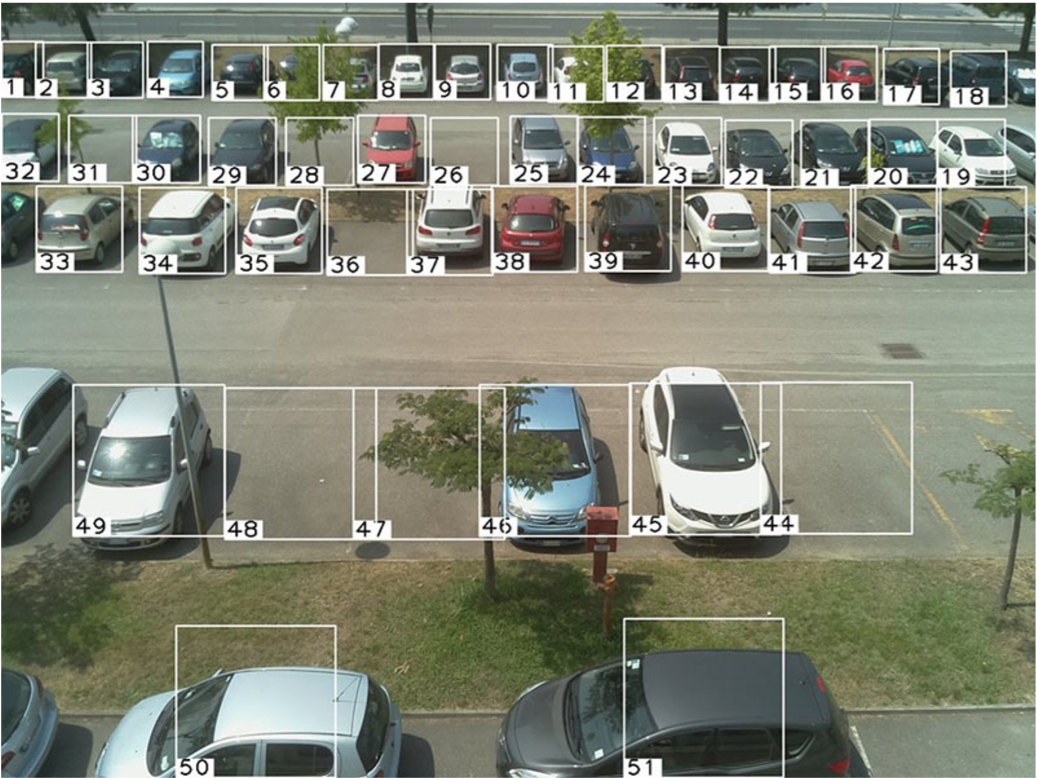
\includegraphics[width=110mm]{img/introduction/dlp_example.png}
    \centering
    \caption{Exemple d'images du corpus utilisé}
    \label{fig:dlp_example}
\end{figure} 

De la même manière, le papier \textit{Parking Stall Vacancy Indicator System Based on Deep Convolutional Neural Networks} permet d'obtenir des résultats similaires. \autocite{paper:psv}

\subsection{Détection des voitures}
Bo Li, Tianfu Wu et Song-Chun présente dans leur papier une méthode de détection de voitures à partir d'image. Ceux-ci utilisent une méthode complexe basées sur des convolutions pour détecter certaines parties des voitures (phares, portes, etc.). Sur le corpus d'images \textit{PKLot}, les résultats atteignent un taux de 55.2\% de réussite. \autocite{paper:car_detect}

\subsection{Conclusions}

En général, le problème de mesure du taux d'occupation d'un parking à l'aide de caméras vidéos est approchée à l'aide d'une segmentation des différentes places de parcs, ce qui est pertinent si les places disponibles sont toutes marquées au sol. Néanmoins, l'approche abordée dans ce travail diffère dans le but de répondre aux problèmes présentés en section \itnameref{intro.contexte} tel que les parkings sauvages. Dans cette optique, on cherchera à détecter les voitures présentes, et non pas à classifier chaque place de parc comme étant libre ou non.

\chapter{Bases technologiques}

\section{Traitement d'images}
\subsection{Représentation d'une image}\label{techno.traitement.repr}
\todo{Aussi parler RGB et HSV}

\subsection{Sous-échantillonnage}
\subsection{Convolution}\label{techno.traitement.convolution}
\todo{Parler du fait qu'on peut séparer chacun des channels de limage pour faire de la convolution, mais qu'on peut 1 séparer, 2 faire la conv séparément, 3 les remettres ensembles}
\subsection{Détection de bord}

\section{Réseau de neurones à convolutions}



\chapter{Conception}


%% ------------------------------------------ %%
%%               ARCHITECTURE                 %%
%% ------------------------------------------ %%
\section{Architecture du système}\label{conception.architecture}

\subsection{Capture des images}
Cette section présente l'architecture du système de capture d'image du parking, nécessaire à ce projet. Une caméra IP sera choisie, qui sera connectée au réseau de la HEIG-VD de la manière décrite ici. La capture d'image a été pensée afin de permettre la connexion de multiples caméras.

Il faudra remarquer que les choix effectués ici non seulement influence la caméra qui sera choisie en section \ref{conception.techno.camera} \nameref{conception.techno.camera}, mais aussi, ces choix dépendent de celle-ci. Ainsi, ces deux travaux (choix de l'architecture de capture d'image et choix de la caméra) ont été réalisés en parallèle.

\subsubsection{Architecture logique}\label{conception.architecture.capture.logique}
%\nomenclature{VM}{machine virtuelle, pour \textit{Virtual Machine} en anglais}
%\newacronym[longplural={Virtual Machines}]{VM}{VM}{Virtual Machine}

%\todo{NOMENCLATURE PAS FONCTIONNEL}

La caméra réseau sera connectée au réseau local de la HEIG-VD. Elle aura donc une adresse IP, qu'il sera possible d'utiliser afin de dialoguer avec elle. Une machine virtuelle (abrégée \textit{VM}, pour \textit{Virtual Machine}) a été mise à disposition de ce projet. Située sur le réseau de l'école, elle permettra de récupérer ses images.

\begin{figure}[!ht]
    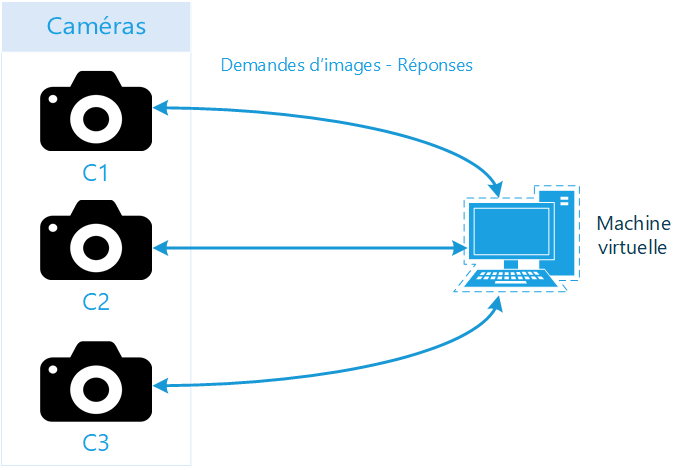
\includegraphics[width=110mm]{img/conception/logic_arch.png}
    \label{fig:capture_cameras}
    \centering
    \caption{Capture d'images de plusieurs caméras}
\end{figure}

La figure \ref{fig:capture_cameras} présente un protocole de demande-réponse sur \textit{HTTP} qui sera utilisé afin de récupérer des images à intervalles réguliers. Il est possible de la préciser ainsi:

\begin{enumerate}
    \item La \textit{VM} émet une requête demandant l'image du parking à une caméra. 
    \item La caméra répond à la \textit{VM} avec ladite image.
\end{enumerate}

Les requêtes et réponses précitées sont fortement dépendantes de la caméra choisie. Ainsi, les détails d'implémentation pourront être trouvés en section \ref{realisation.capture} \nameref{realisation.capture}.


\subsubsection{Architecture physique}\label{conception.architecture.camera.physique}
\paragraph{Positionnement de la caméra}\label{conception.architecture.camera.physique.position}
La caméra doit pouvoir être capable de capturer des images de parking. Pour ce faire, une caméra sera installée sur le toit de la HEIG-VD. 

Il faut remarquer que l'installation de périphériques sur la terrasse n'y ai pas des plus aisés. De plus, l'édification d'une salle de conférence y a débuté en date du 26 février 2018\footnote{informations tirées d'un mail envoyé aux collaborateurs et étudiant de la HEIG-VD}, ne facilitant pas l'installation. Il en sera tenu compte lors du choix de la caméra. Plus d'informations concernant l'installation de celle-ci est disponible en section \ref{realisation.capture} \nameref{realisation.capture}.

\paragraph{Connexion de la caméra}

Ici, deux points sont principalement étudier: l'alimentation de la caméra, et sa connexion au réseau local de la HEIG-VD.  

\begin{figure}[H]
    
\includegraphics[width=110mm]{img/conception/cam_con_1.png}
    \label{fig:cam_connection_1}
    \centering
    \caption{Caméra alimentée et connectée au réseau par câble}
\end{figure}

La caméra pourrait être câblée au réseau électrique, ainsi qu'au réseau local. Il est nécessaire de tirer 2 câble, à 2 endroits différents: l'un au réseau électrique, et l'autre à un switch ou une prise Ethernet présente dans le bâtiment.

\begin{figure}[H]
    
\includegraphics[width=110mm]{img/conception/cam_con_2.png}
    \label{fig:cam_connection_2}
    \centering
    \caption{Caméra câblée au réseau et alimentée par \textit{PoE}}
\end{figure}

Elle pourrait aussi être câblée uniquement au réseau local. En effet, il serait possible de profiter de la technologie \textit{Power over Ethernet} (\textit{PoE}) permet de fournir en électricité un périphérique réseau via le câble Ethernet. Il faut cependant noter que le switch connecté à la caméra doit pouvoir fournir cette possibilité.

\begin{figure}[H]
    
\includegraphics[width=110mm]{img/conception/cam_con_3.png}
    \label{fig:cam_connection_3}
    \centering
    \caption{Caméra alimentée par câble et connectée au réseau en Wifi}
\end{figure}

La caméra pourrait être connectée au réseau électrique par câble. La connexion au réseau local pourrait être effectuée par Wifi. Il faut cependant noter que le Wifi doit être puissant et fiable: la caméra, installé à l'extérieur du bâtiment, pourrait ne pas capter suffisamment un signal provenant de l'intérieur, ceci dû aux larges murs en bêton. 

\begin{figure}[H]
    
\includegraphics[width=110mm]{img/conception/cam_con_4.png}
    \label{fig:cam_connection_4}
    \centering
    \caption{Caméra auto-alimentée et connectée en Wifi}
\end{figure}

Une batterie, ou un panneau solaire, pourrait l'alimenter. Munie du Wifi, cette solution ne demanderait aucun câblage. On notera cependant que le prix d'un tel équipement pourrait être élevé.

\subparagraph{Solution choisie}

Comme indiqué au paragraphe \nameref{conception.architecture.camera.physique.position}, la construction d'une salle pourrait compromettre l'installation de câble. C'est pourquoi une caméra auto-suffisante sera préférée. Ainsi, la caméra devra pouvoir fournir:
\begin{itemize}
    \item Une connexion à un signal Wifi puissante et fiable
    \item Elle sera auto-alimentée. De préférence, un panneau solaire sera utilisé afin que des changements de batteries ne soit pas nécessaire.
\end{itemize}

\subsection{Distribution des informations à l'utilisateur}

%% ------------------------------------------ %%
%%           CHOIX TECHNOLOGIQUES             %%
%% ------------------------------------------ %%

\section{Choix technologiques}

\subsection{Caméra réseau}\label{conception.techno.camera}
Une caméra réseau fournissant des images de qualités, et ce dans un prix raisonnable, est nécessaire dans ce projet afin de capturer des images. Celle-ci sera utilisée principalement dans 2 buts, précisés ci-après.

\paragraph{Entrainement du modèle}
Dans un premier temps, il s'agit d'entrainer le modèle à partir des images fournies par la caméra. Pour ce faire, il doit être possible de capturer des photos à intervalles réguliers. Ces images seront ensuite annotées, puis utilisées pour entrainer le modèle du réseau de neurones à convolutions. 

\paragraph{Utilisation du modèle}
Une fois le modèle définit, le but de ce projet est de l'utiliser afin de détecter le nombre de voiture présentes courant sur le parking. Ainsi, dans un second temps, la caméra doit pouvoir fournir des images du parking "en direct", dans le but d'obtenir un état courant du parking. Il faut noter qu'ici, la notion "en direct" signifie "relativement court", soit de l'ordre de la minute. En effet, en tant qu'utilisateur, obtenir le taux d'occupation du parking à la minute près semble suffisant. Bien entendu, un intervalle plus court entre chaque prise, ou un flux vidéo, est un plus.

Il convient donc d'effectuer l'achat d'une caméra permettant le bon déroulement de ce projet. Pour ce faire, plusieurs caméras ont été évaluées. On rencontrera donc dans les prochaines sections les contraintes et critères nécessaires à une bonne évaluation. Les caméras seront notées, ce qui permettra d'en retirer celle qui convient le mieux à ce projet.

Il est important de noter qu'idéalement, des tests en condition réelles des différentes caméras auraient dû être effectués. Cependant, dans le cadre de ce travail de Bachelor, le budget mis à disposition ne peut le permettre. C'est pourquoi une seule caméra sera choisie sur la base des critères définis.

\subsubsection{Contraintes}\label{conception.techno.camera.contraintes}
Comme vu en section \ref{conception.architecture.camera.physique}, installer une caméra sur le toit de la HEIG-VD a pour conséquence que certaines contraintes, tant d'ordre techniques qu'organisationnelles, doivent être respectées. Celles-ci sont explicitées dans cette section.

\paragraph{Capture d'images}
La caméra devra au minimum permettre la capture d'images à intervalles réguliers d'une façon ou d'une autre. L'intervalle minimum de capture est de l'ordre de la minute, afin de pouvoir obtenir l'état courant du parking filmé. La capture de vidéos n'est pas nécessaire. On notera que si celle-ci ne fournit malheureusement que la fonctionnalité de capture vidéo, il serait tout de même possible d'en extraire des images utilisables. 

\paragraph{Usage extérieur}
La caméra doit être prévue pour un usage extérieur, avec une protection contre les intempéries (pluie, neige, froid, chaud, etc.)

\paragraph{Connexion réseau}
En lien avec le paragraphe précédent, la caméra doit nécessairement avoir une interface Wifi permettant de se connecter au réseau de l'école. Une connexion par Ethernet n'est pas envisageable.

\paragraph{Caméra auto-alimentée}
Comme vu en section \ref{conception.architecture.camera.physique}, la caméra doit être auto-alimentée et non câblée. Ainsi, une combinaison de batteries et de panneaux solaires semble être idéal. On peut noter que l'utilisation de batteries uniquement est envisageable dans le cadre d'un prototypage, mais ce uniquement si le remplacement de celles-ci doit être effectué à intervalles relativement éloignés, de l'ordre de la semaine.

\paragraph{Résolution d'image}
Dans le but d'obtenir des images de qualités suffisantes, la résolution de l'image capturées devra nécessairement être d'au minimum 1280x720 pixels.

\subsubsection{Critères}
Plusieurs critères, ont été définis. Chacune des caméras retenues seront notées selon ceux-ci. On les trouvera ci-après, où leur pondération sont indiqués entre crochets ([]). Une pondération élevée signifie une plus grande importance de ce critère.

\paragraph{Qualité d'image [1]}
La caméra doit avoir une bonne qualité d'image. On jugera:
\begin{itemize}
    \item La résolutions de l'image. Celle-ci doit être d'au minimum 1280x720 pixels.
    \item La qualité de l'image (si possible).
\end{itemize}

\paragraph{Fonctionnalités réseaux [2]}
La caméra doit pouvoir fournir des images via le réseau et il doit être possible d'en récupérer à intervalles réguliers. Pour ce faire, on pensera à des protocoles comme les suivants: 
\begin{description}
    \item[ONVIF (Open Network Video Interface Forum)] Standard industriel ouvert permettant de contrôler, configurer et communiquer avec des caméras de sécurité IP. Permet notamment la lecture de flux vidéo en temps réel et la capture de photos \autocite{wiki:onvif}
    \item[RTSP (Real Time Streaming Protocol)] Développé par RealNetworks, Netscape et Columbia University, protocole de communication permettant de lire en temps réel un flux vidéo. \autocite{wiki:RTSP}
    \item[Requêtes HTTP] Il pourrait être possible de capturer et de récupérer à la demande une photo à l'aide de requêtes HTTP.
    \item[Flux sur HTTP] Permet la lecture de flux vidéo sur HTTP en s'appuyant sur des formats tel que MPEG-4.
    \item[Interface Web HTTP] Permet la configuration de la caméra IP via un serveur Web qu'elle expose. 
    \item[FTP] La caméra peut exposer un serveur FTP contenant les photos capturées. Elle pourrait aussi téléverser des photos capturées sur un serveur FTP distant.
On notera avant tout sur la facilité d'utilisation des différents protocoles.
\end{description}

\paragraph{Fonctionnement auto-alimenté [4]}
La caméra doit être auto-alimentée et non câblée. Comme critères, on pensera donc à:
\begin{itemize}
    \item La durée de vie de la caméra en fonctionnement auto-alimenté. Idéalement, la caméra ne devrait nécessiter aucune intervention humaine.
    \item La portée du Wifi. La puissance du signal doit être assez forte afin de pouvoir capter les bornes Wifi de l'école depuis le toit de la HEIG-VD. Il est important de noter que ce critère peut être difficilement évalué avant l'achat de la caméra.
\end{itemize}

\paragraph{Capture de photo [2]}
La caméra doit être capable de fournir un moyen pour capturer des photos à intervalles réguliers, de l'ordre de la minute. Pour ce faire, la caméra peut fournir un système de capture de photos automatique, ce qui est un plus. On évaluera donc les moyens fournis par la caméra permettant ces captures.

\paragraph{Angle de vue [2]}
L'angle de vue de la caméra doit être suffisamment grand afin d'obtenir une image du parking dans son ensemble. Il peut être suffisant à partir de 40°, de par la hauteur à laquelle elle sera placée. Cependant, un angle de 90° semble plus satisfaisant. Ces angles ont été définis à l'aide des informations fournies par \url{videosurveillance-boutique.fr} \autocite{cam:securite_info}.

\paragraph{Vision de nuit [1]}
Idéalement, la caméra devrait pouvoir fournir une vision de nuit afin de pouvoir capturer des images de parking par toute heure. On pensera notamment aux matinées et aux soirées d'hiver, où les véhicules arrivent et partent alors que la luminosité est encore très faible. Cependant, dans le cadre de ce TB, cette fonctionnalité n'est pas strictement nécessaire.

\paragraph{Facilité d'installation [1]}
La facilité d'installation de la caméra sera prise en compte. On pensera aux dimensions de celle-ci, à son poids, au nombre de ses composants (par exemple, est-il nécessaire d'installer une batterie en plus de la caméra, ou est-elle incorporée à celle-ci?), ou encore aux accessoires fournis pour son installation. 

\paragraph{Prix [4]} Bien évidemment, le prix doit entrer en ligne de compte. 100.- CHF sera indiqué comme prix maximum afin d'obtenir la meilleure note. A partir de 500.- CHF, on évaluera ce prix comme étant mauvais.

\subsubsection{Caméras disponibles et évaluation}
Bien que la surveillance n'est pas un but de ce TB, les caméras de sécurités semblent être les plus adaptées. En effet, elles fournissent généralement des fonctionnalités de capture de photos, de connexion réseau, de vision de nuit, possèdent un angle de vue suffisant et sont souvent résistantes à un environnement extérieur. De plus, elles sont spécialement conçues pour un usage qui s'apparente à celui qui de ce TB, et sont donc adaptées à la prise d'images de parking.

L'achat distinct d'une caméra, de panneaux solaires et de batteries est envisageable. Néanmoins, dans un premier temps, seuls des kits complets (caméra, batteries, panneaux solaires) ont été analysés. En effet, l'installation et le choix des différents composants nécessaires à un système solaire complet semble difficile lorsqu'on est pas du domaine, et des problèmes d'interopérabilité pourraient survenir. Ceci reste cependant une solution viable si aucun kit ne correspond aux contraintes définies.

De part les contraintes très spécifiques précisées jusqu'ici, le nombre de caméras les satisfaisant toutes sont peu nombreuses. On trouvera ci-après les kits complets solaires auto-suffisants qui ont été évalués. Il faut aussi noter que seules les caméras les plus appropriées sont indiquées ici.

\paragraph{\textbf{Electrosun} -- Caméra-surveillance-solaire}
\textit{Electrosun} est une entreprise de domotique solaire française. Entre autres, un kit solaire de caméra complet est mis en vente. \autocite{cam:electrosun_site}

\begin{figure}[ht]
    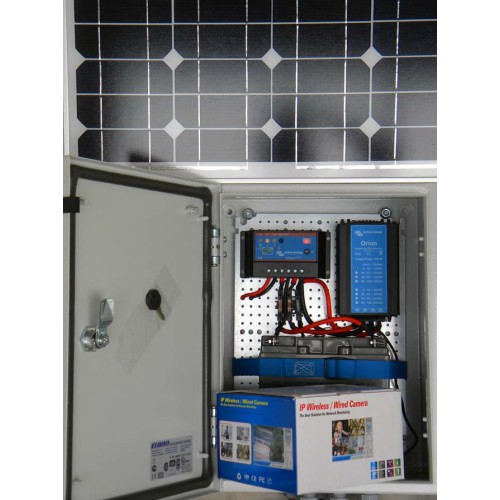
\includegraphics[width=50mm]{img/conception/electrosun_cam.jpg}
    \centering
    \captionsource{\textbf{Electrosun} Caméra de surveillance solaire}{cam:electrosun_site}
\end{figure}

Bien qu'elle satisfasse la plupart des contraintes, elle n'a pas été retenue pour l'évaluation. En effet, la résolution des images capturées n'est que de 640x480 pixels, ce qui n'est pas suffisant.

\paragraph{\textbf{Reolink} -- Argus 2}
L'entreprise \textit{Reolink} développe des caméras 100\% sans fil, avec batteries rechargeables et panneaux solaires. Elle est auto-suffisante.\autocite{cam:argus2}

\begin{figure}[ht]
    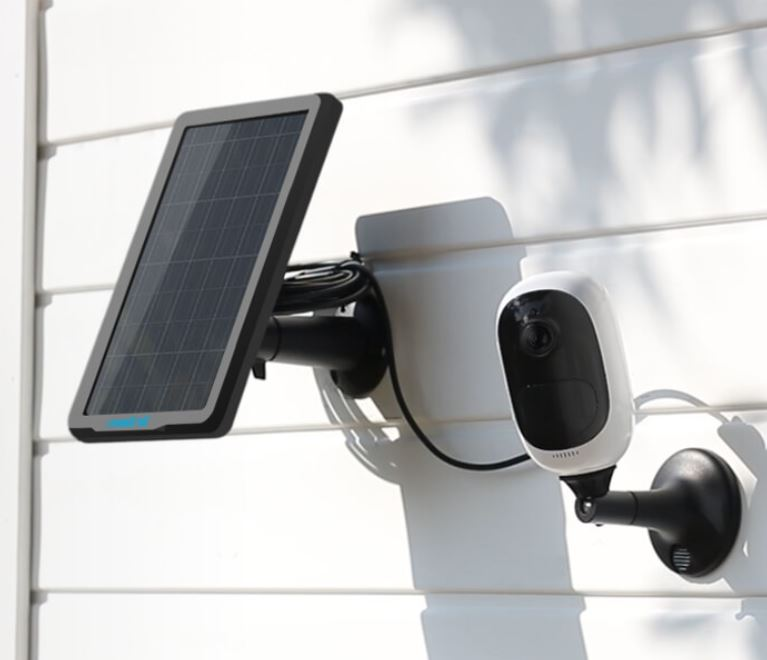
\includegraphics[width=50mm]{img/conception/argus2_cam.jpg}
    \centering
    \captionsource{\textbf{Reolink} Argus 2}{cam:argus2}
\end{figure}

Elle permet de capturer des photos FullHD (1920x1080 pixels), possède une fonction de vision de nuit ou encore, l'utilisation en extérieur est possible. Cependant, cette caméra n'a elle non plus pas pu être prise en considération. En effet, elle a été pensée pour un usage privé, et bien que la caméra puisse être connectée à un réseau Wifi, l'accès à celle-ci n'est possible qu'à l'aide d'une application smartphone (tel que décrit dans les spécifications disponibles sur le site officiel \url{https://reolink.com/product/argus-2}\autocite{cam:argus2}). Récupérer des photographies à intervalles réguliers semble donc difficilement réalisable.

\paragraph{\textbf{Wanscam} -- HW0029-3}

\textit{Wanscam} est une entreprise chinoise spécialisées dans la production de caméra réseau. Plusieurs versions de son modèle \textit{HW0029} sont disponibles. Ici est présenté le modèle \textit{HW0029-3}. \autocite{cam:wan3}

\begin{figure}[ht]
    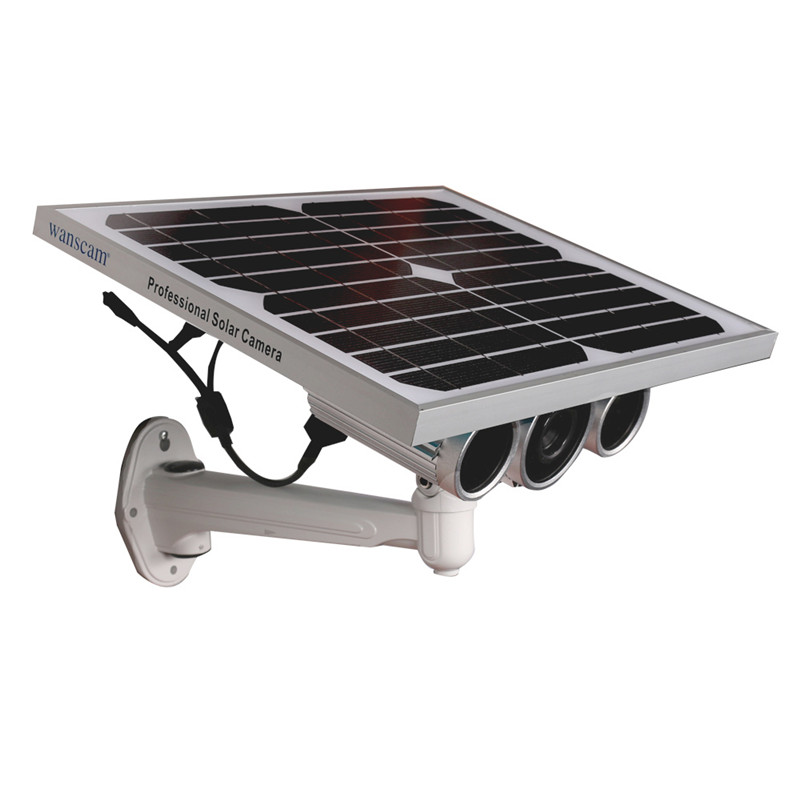
\includegraphics[width=50mm]{img/conception/wan3_cam.jpg}
    \centering
    \captionsource{\textbf{Wanscam} HW0029-3}{cam:wan3}
\end{figure}

Cette caméra satisfait toutes les contraintes définies en section \ref{conception.techno.camera.contraintes}. On trouvera en table \ref{tab:HW0029-3} ses principales caractéristiques.\footnote{Tirées des spécifications officielles \autocite{cam:wan3} et d'un test indépendant \autocite{cam:wan3-test}.}

\begin{table}[H]
    \centering
    \caption{Caractéristiques de la caméra \textbf{Wanscam} \textit{HW0029-3}}
    \label{tab:HW0029-3}
    \begin{tabular}{@{}ll@{}}
    \toprule
    Caractéristique        & Valeurs                                                                                                                                                                                                                                                                                     \\ \midrule
    Image                  & 1280 x 720, 25fps, compression H.264                                                                                                                                                                                                                                                        \\ [0.8ex]
    Angle de vue           & 40°                                                                                                                                                                                                                                                                                         \\ [0.8ex]
    Vision nocturne         & Visibilité jusqu'à 15 mètres                                                                                                                                                                                                                                                                \\ [0.8ex]
    Réseau                 & RJ45, Wifi 802.11 b/g/n                                                                                                                                                                                                                                                                     \\ [0.8ex]
    Auto-alimentation      & \begin{tabular}[c]{@{}l@{}}2 batteries de 12A et panneau solaire. \\ Sans soleil: 48h d'utilisation. \\ Faible température (\textless 26°) des rayons de soleil: 7 jours d'utilisations. \\ Grande température (\textgreater 33°) des rayons de soleil: fonctionnement continu\end{tabular} \\ [0.8ex]
    Stockage               & Carte MicroSD de 16Gb incluse, support jusqu'à 128Gb                                                                                                                                                                                                                                        \\ [0.8ex]
    Détection de mouvement & Oui                                                                                                                                                                                                                                                                                         \\ [0.8ex]
    Accès aux images       & Flux HTTP, ONVIF, RTSP, requêtes HTTP                                                                                                                                                                                                                                                       \\ [0.8ex]
    Dimensions et poids    & 370x290x110 mm, 2.7 kg                                                                                                                                                                                                                                                                      \\ \bottomrule
    \end{tabular}
\end{table}

On notera que le panneau solaire est fixé sur la caméra. Ainsi, dans le but de garder une exposition au soleil suffisante, l'angle de la caméra ne doit pas être trop élevé. Il y a donc certaines contraintes à l'installation de celle-ci.

Concernant la capture d'image, la caméra fournit des \textit{endpoints HTTP} (dont une liste peut être trouvée sur le site \url{tutoriels.domotique-store.fr}\autocite{cam:wan3-url}) permettant de récupérer l'image actuelle. Il est donc facile d'imaginer un simple agent qui, à intervalle régulier, demandera à la caméra une image, et l'enregistrera en local.

Les caméras \textbf{Wanscam} ne sont pas des plus faciles à trouver dans le commerce. Elles sont principalement disponibles sur \url{aliexpress.com}. Le modèle \textit{HW0029-3} peut être trouvé à partir de 170CHF (en date du 09.03.2018, \url{aliexpress.com}).

La grille d'évaluation \ref{cam:wan3_eval} a pu être remplie à l'aide de ces spécifications.

\begin{table}[H]
    \centering
    \caption{Evaluation de la caméra \textbf{Wanscam} \textit{HW0029-3}}
    \label{cam:wan3_eval}
    \begin{tabular}{@{}llp{8cm}@{}}
        \toprule
        Critère                              & Note (de 1 à 5) & Remarque                                                                                                                                                                   \\ \midrule
        Qualité d'image              & 3 [1]               & La qualité d'image semble suffisante selon les tests effectué par \url{lesbonstuyauxgeeks.fr}\autocite{cam:wan3-test}. La résolution est de 1280x720 pixels, ce qui est suffisant. \\ [0.8ex]
        Fonctionnalités réseaux      & 5 [2]              & La caméra offre notamment un endpoint HTTP sur lequel récupérer les images.                                                                                                \\ [0.8ex]
        Fonctionnement auto-alimenté & 4 [4]              & La caméra est totalement auto-suffisante s'il y a assez de soleil. On notera cependant le panneau solaire fixe qui peut nuire à l'exposition du soleil. Elle supporte le Wifi 802.11n: à première vue, le signal semble suffisant.                   \\ [0.8ex]
        Capture de photo             & 5 [2]              & Il est facile de récupérer des images sur cette caméra. Elle offre en plus un système de capture de photos à intervalles réguliers automatique. Elle offre aussi la possibilité de récupérer un flux vidéo.                            \\ [0.8ex]
        Angle de vue                 & 1 [2]              & Un angle de vue de 40° semble tout juste suffisant.                                                                                                                        \\ [0.8ex]
        Vision de nuit               & 2 [1]               & Elle fournit une vision nocturne à 15m. Il est cependant possible d'ajouter des LED infrarouges supplémentaires afin d'obtenir une meilleure vision de nuit\autocite{cam:wan3-url}. \\ [0.8ex]
        Facilité d'installation      & 3 [1]              & La caméra mesure jusqu'à 37 cm, ce qui nuit à sa facilité d'installation. De plus, le panneau solaire est fixe, ce qui contraint la position et l'angle de la caméra.      \\ [0.8ex]
        Prix                         & 4 [4]              & A partir d'environ 170.- CHF \\ \midrule
        && \textbf{Note finale: 3.6/5} \\ \bottomrule
    \end{tabular}
\end{table}

\paragraph{\textbf{Wanscam} -- HW0029-5}
Le modèle \textit{HW0029-3} de \textbf{Wanscam} est la nouvelle version du modèle \textit{HW0029-3} décrit précédemment. Elle possède la plupart des mêmes caractéristiques, mais propose une meilleure résolution (1920x1080), des batteries à plus grande capacité, un meilleur champ de vision, ou encore, une vision de nuit accrue jusqu'à 100m. Son prix est cependant plus élevé que la caméra \textit{HW0029-3}. Les caractéristiques indiquées dans ce rapport proviennent du site officiel \url{wanscam.com}\autocite{cam:wan5}.

\begin{figure}[ht]
    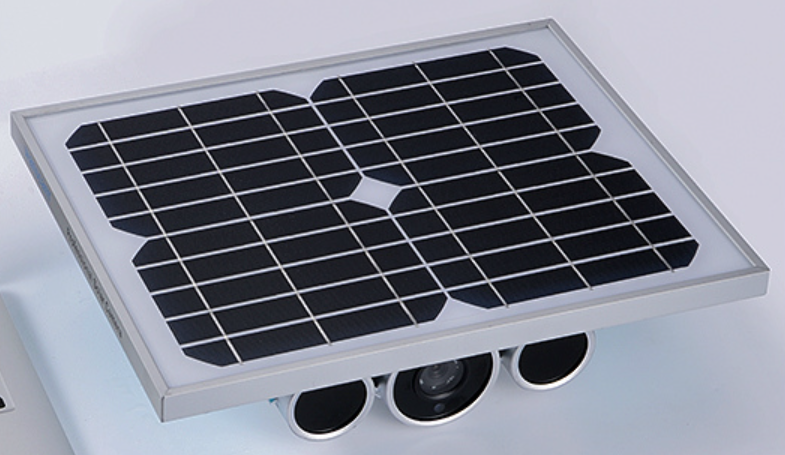
\includegraphics[width=50mm]{img/conception/wan5_cam.png}
    \centering
    \captionsource{\textbf{Wanscam} HW0029-5}{cam:wan5}
\end{figure}

\begin{table}[H]
    \centering
    \caption{Caractéristiques de la caméra \textbf{Wanscam} \textit{HW0029-5}}
    \label{tab:HW0029-5}
    \begin{tabular}{@{}ll@{}}
    \toprule
    Caractéristique        & Valeurs                                                                                                                                                                                                                                                                                     \\ \midrule
    Image                  & 1920 x 1080, 25-30fps, compression H.264                                                                                                                                                                                                                                                        \\ [0.8ex]
    Angle de vue           & 80°                                                                                                                                                                                                                                                                                         \\ [0.8ex]
    Vision nocturne         & Visibilité jusqu'à 100 mètres                                                                                                                                                                                                                                                                \\ [0.8ex]
    Réseau                 & RJ45 100Mbps, Wifi 802.11 b/g/n                                                                                                                                                                                                                                                                     \\ [0.8ex]
    Auto-alimentation      & \begin{tabular}[c]{@{}l@{}}2 batteries de 12A et panneau solaire. \\ Sans soleil: 54h d'utilisation. \end{tabular} \\
    Stockage               & Carte MicroSD de 16Gb incluse, support jusqu'à 128Gb                                                                                                                                                                                                                                        \\ [0.8ex]
    Détection de mouvement & Oui                                                                                                                                                                                                                                                                                         \\ [0.8ex]
    Accès aux images       & Flux HTTP, ONVIF, RTSP, requêtes HTTP                                                                                                                                                                                                                                                       \\ [0.8ex]
    Dimensions et poids    & 370x286x960 mm, 4.3 kg                                                                                                                                                                                                                                                                      \\ \bottomrule
    \end{tabular}
\end{table}

Il faudra noter que cette caméra est plus lourde, bien que plus petite, que le précédent modèle. 

De ces caractéristiques, il a été possible d'évaluer cette caméra dans la grille d'évaluation \ref{cam:wan5_eval} 

\begin{table}[H]
    \centering
    \caption{Evaluation de la caméra \textbf{Wanscam} \textit{HW0029-5}}
    \label{cam:wan5_eval}
    \begin{tabular}{@{}llp{8cm}@{}}
        \toprule
        Critère                      & Note (de 1 à 5) & Remarque                                           \\ \midrule
        Qualité d'image              & 4 {[}1{]}       & La qualité de l'image est meilleure que le modèle précédent, avec une résolution de 1920x1080 pixel.                                                              \\ [0.8ex]
        Fonctionnalités réseaux      & 5 {[}2{]}       & La caméra offre notamment un endpoint HTTP sur lequel récupérer les images.                                                                                       \\ [0.8ex]
        Fonctionnement auto-alimenté & 4 {[}4{]}       & De la même manière que le modèle précédent, la caméra est totalement auto-suffisante s'il y a assez de soleil. Sans soleil, elle est auto-suffisante jusqu'à 54h. Elle support la norme Wifi 802.11n \\ [0.8ex]
        Capture de photo             & 5 {[}2{]}       & Il est facile de récupérer des images sur cette caméra. De plus, elle offre un système de capture de photos à intervalles réguliers automatiques. Elle offre aussi la possibilité de récupérer un flux vidéo.                  \\ [0.8ex]
        Angle de vue                 & 4 {[}2{]}       & Un angle de vue de 80° semble être approprié pour ce projet. Un angle supérieur n'aurait pas été superflu.                                                        \\ [0.8ex]
        Vision de nuit               & 5 {[}1{]}       & Elle fournit une vision nocturne à 100m.                                                                                                                          \\ [0.8ex]
        Facilité d'installation      & 3 {[}1{]}       & Tout comme le modèle HW0029-3, la caméra n'est pas des plus petites, mesurant jusqu'à 37 cm. Le panneau solaire est fixé à la caméra.                             \\ [0.8ex]
        Prix                         & 3 {[}4{]}       & A partir d'environ 230.- CHF   \\ \midrule
        && \textbf{Note finale: 4.0/5} \\ \bottomrule
    \end{tabular}
\end{table}

\subparagraph{Remarque} Le modèle \textbf{Wanscam} \textit{HW0029-4} (ainsi que sa version améliorée \textit{HW0029-6}) n'a pas été pris en compte. En effet, il fourni en plus un système de puce 4G afin de pouvoir connecter la caméra à un réseau mobile. En conséquence, le prix est trop élevé, dépassant les 400.- CHF.

\paragraph{\textbf{Visortech} -- Caméra Solaire IP}
Cette caméra satisfait toutes les contraintes définies dans la section \ref{conception.techno.camera.contraintes} \nameref{conception.techno.camera.contraintes}. Ses caractéristiques principales sont décrites à la table \ref{tab:visortech_spec}. Il a été possible de remarquer que la caméra décrite ici est disponible sous différents noms, comme \textit{IdealSmartCam}.

\begin{figure}[ht]
    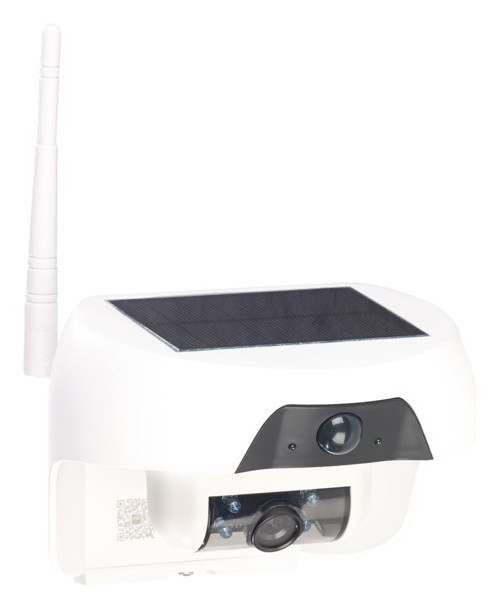
\includegraphics[width=50mm]{img/conception/visortech_cam.jpg}
    \centering
    \captionsource{Caméra Visortech}{cam:visortech}
\end{figure}

On notera le peu d'information disponible concernant les spécifications de cette caméra. Par exemple, il est difficile de connaitre les méthodes disponibles afin de pouvoir récupérer des images depuis le réseau local, tant et si bien que cela soit possible. On notera que le vendeur a été contacté, sans réponse de sa part.

\begin{table}[H]
    \centering
    \caption{Caractéristiques de la caméra \textit{Visortech}}
    \label{tab:visortech_spec}
    \begin{tabular}{@{}lp{10cm}@{}}
    \toprule
    Caractéristique        & Valeurs                                                          \\ \midrule
    Image                  & 1280 x 720, compression H.264. Prise de vue en continu possible. \\ [0.8ex]
    Angle de vue           & 90°                                                              \\ [0.8ex]
    Vision nocturne         & Visibilité jusqu'à 5 mètres                                      \\ [0.8ex]
    Réseau                 & Wifi 802.11 b/g/n                                                \\ [0.8ex]
    Auto-alimentation      & Panneau solaire intégré de 0.8 Watt, jusqu'à 5 jours sans soleil. Auto-suffisante.     \\ [0.8ex]
    Détection de mouvement & Oui                                                              \\ [0.8ex]
    Dimensions et poids    & 161x155x108 mm, 0.8 kg                                            \\  [0.8ex]\bottomrule
    \end{tabular}
\end{table}

Malgré le manque d'information, cette caméra a tout de même été évaluée. Il sera de ce fait possible de savoir si elle peut être un choix viable, ou non. La grille d'évaluation correspondante peut être trouvée en table \ref{tab:visortech_eval}

\begin{table}[H]
    \centering
    \caption{Evaluation de la caméra \textit{Visortech}}
    \label{tab:visortech_eval}
    \begin{tabular}{@{}llp{8cm}@{}}
        \toprule
        Critère                      & Note (de 1 à 5) & Remarque                          \\ \midrule
        Qualité d'image              & 3 {[}1{]}       & Sa résolution est de 1280x720 pixel.                                                                                                  \\ [0.8ex]
        Fonctionnalités réseaux      & 2 {[}2{]}       & Accès via smartphone possible, peu d'informations concernant les protocoles réseaux disponibles.                                      \\ [0.8ex]
        Fonctionnement auto-alimenté & 3 {[}4{]}       & Devrait être auto-suffisante. Cependant, informations peu claires si prises d'images en continu. Accepte la norme Wifi 802.11n. \\ [0.8ex]
        Capture de photo             & 3 {[}2{]}       & Permet l'accès au flux vidéo en direct. Peu d'informations sur les protocoles disponibles.                                            \\ [0.8ex]
        Angle de vue                 & 5 {[}2{]}       & Angle de vue de 90°. Meilleur champ de vision parmi les caméras évaluées.                                                              \\ [0.8ex]
        Vision de nuit               & 2 {[}1{]}       & Elle fournit une vision nocturne à 5m.                                                                                                \\ [0.8ex]
        Facilité d'installation      & 3 {[}1{]}       & La caméra est relativement petite, et ne pèse que 850g. On notera l'absence de pied: une fixation à un mur semble nécessaire.         \\ [0.8ex]
        Prix                         & 3 {[}4{]}       & A partir d'environ 220.- CHF                                                                                                          \\ [0.8ex]
                                    &                 & \textbf{Note finale: 3.1/5} \\ \bottomrule
    \end{tabular}
\end{table}

\subsubsection{Choix final}

La caméra \textit{Visortech} arrive dernière du classement, avec une note de 3.1. Ceci est avant tout du au manque d'information sur les protocoles utilisables afin de récupérer via le réseau des images. Elle n'a donc pas été retenue.

\begin{table}[!ht]
    \centering
    \caption{Caméras - Synthèse des résultats}
    \label{cam:synthese}
    \begin{tabular}{@{}lll@{}}
    \toprule
      & Caméra           & Note \\ \midrule
    \textbf{1} & Wanscam HW0029-5 & 4.0  \\
    \textbf{2} & Wanscam HW0029-3 & 3.6  \\
    \textbf{3} & Visortech        & 3.1  \\ \bottomrule
    \end{tabular}
\end{table}

Les deux versions de la caméra \textit{HW0029} de \textbf{Wanscam} montrent des résultats proches. Elles sont avant tout distinguable par leur qualité d'image, leur vision de nuit, leur durée de fonctionnement sur batterie et leur angle de vue, où toutes ses caractéristiques sont améliorées sur le nouveau modèle (\textit{HW0029-5}). Ainsi, seul le rapport qualité/prix peut faire pencher la balance d'un côté ou d'un autre. Avec un peu de recherche, la version \textit{HW0029-5} a été trouvée à 187.50€ sur \url{aliexpress.com}\autocite{cam:wan5-buy} (frais de livraison inclus), soit 225.- CHF (1.17CHF/€ en date du 13 mars 2018\autocite{util:cours}, arrondi au dixième supérieur, soit 1.20 CHF/€). 

Au prix indiqué plus haut, et vis-à-vis du classement présenté en table \ref{cam:synthese}, la caméra \textbf{Wanscam} \textit{HW0029-5} a été choisie pour la capture d'image que demande ce projet.

\subsection{Langage de développement}
Afin de choisir le langage de programmation qui sera majoritairement utilisé dans ce projet, il est premièrement nécessaire de définir quel en sera son utilisation. On résumera donc ses objectifs principaux ainsi:
\begin{itemize}
    \item Le langage sera utilisé afin de capturer des images sur HTTP.
    \item Le langage sera fortement utilisé pour du traitement d'image.
    \item Le langage sera fortement utilisé pour du \textit{Machine Learning}, plus spécifiquement des réseaux de neurones à convolutions.
\end{itemize}

De ce fait, se tourner vers un langage s'approchant du \textit{script} (qu'on pourra par exemple opposer au langage \textit{Java}) semble avoir plusieurs avantages:
\begin{itemize}
    \item Le langage sera beaucoup utilisé afin de traiter des informations. Ces traitements seront relativement courts, mais multiples. Un langage de script semble suffisant.
    \item Les langages de scripts sont légers, aisément maintenables et évolutifs. Il est cependant important de noter qu'ils le sont seulement si les programmes développés restes courts et bien construit. 
    \item Les scripts ressemblent souvent à de la programmation procédurale, ce qui peut en faciliter son écriture. Puisqu'avant tout, des traitements seront effectués, un style de programmation procédurale semble idéal.
\end{itemize}

Dans le cadre de ce TB, du \textit{Machine Learning} sera effectué. Il convient donc aussi de s'informer sur les langages de développement les plus populaires utilisés dans ce contexte. On en tirera une liste, non-exhaustive. Il faut noter que cette liste a été définie par ce qui a pu être vu par l'expérience, et non par un réel classement:
\begin{description}
    \item[R] Environnement gratuit de statistiques et graphiques.\autocite{lang:R}
    \item[MATLAB] Développé par \textit{MathWorks}, combine un environnement \textit{desktop} pour de l'analyse et un langage de programmation spécialisés.\autocite{lang:matlab}
    \item[Python] Langage de programmation permettant un développement rapide et efficace. \autocite{lang:python}
\end{description}

Le choix du langage dépend aussi fortement des librairies qui sont disponibles et utilisées. Dans le cadre du \textit{Machine Learning} et du traitement d'images, elles sont très souvent disponibles en \textit{Python}.

\paragraph{Choix du langage}
De part ce qui a été précisé précédemment, \textit{Python} semble être le langage idéal.

\paragraph{Limitation}
Une des principales limitations de ce langages et qu'il est interprété. Ainsi, les performances peuvent être plus faible qu'un langage compilé\footnote{ On notera cependant qu'il est possible, si on le souhaite, de compiler du \textit{Python}. Là n'est cependant pas son but premier}. Cependant, et comme on le verra plus tard, les librairies fournies sont souvent des \textit{wrappers} interfaçant du code compilé. Ainsi, les traitements lourds sont souvent efficaces, où \textit{Python} peut ne servir qu'à connecter des composants et définir des configurations. 

\subsection{Traitement d'images}
Dans ce projet, une des premières étapes consiste à traiter les images provenant de la caméra afin qu'elles puissent être utilisées convenablement dans l'algorithme de \textit{Machine Learning}. On trouvera ci-après les différents traitements qui doivent pouvoir être réalisés:
\begin{description}
    \item[\textit{Downsampling}] L'image reçue de la caméra sera sous-échantillonnée.
    \item[\textit{Edge detection}] Les bords pouvant être détectés dans l'image devront pouvoir être mis en valeur. 
\end{description}

\subsubsection{Librairies disponibles}
Plusieurs librairies \textit{Python} sont disponibles. Ici en sont décrites deux.

\paragraph{OpenCV}
OpenCV\autocite{lib:opencv} (Open Source Computer Vision Library) est une librairie Open Source permettant le traitement d'image. Elle peut être utilisée en C++, Java, et Python. Elle est écrite en C/C++ est et optimisée pour une utilisation sur un CPU multi-core. Elle permet notamment de sous-échantillonner une image et de détecter des bords, mais possède aussi beaucoup de fonctionnalités liées au \textit{Machine Learning}.

\paragraph{Scikit-image}
Scikit-image\autocite{lib:skimage}, abrégé \textit{skimage}, est une collection gratuite et Open Source d'algorithmes pour le traitement d'images en python. Elle permet aisément de sous-échantillonner des images, ainsi que de détecter des bords à l'aide de filtre prédéfini (convolutions).

\subsubsection{Comparaison}
Les deux librairies pré-citées sont ressemblantes sur bien des points. Une image, dans les deux cas, est représentée sous la forme d'un tableau \textit{numpy}\footnote{Numpy est une librairie scientifique permettant d'utiliser en \textit{Python} des tableaux multidimensionnels de manière efficaces.\autocite{lib:numpy}} à 3 dimensions. La syntaxe des deux librairies sont aussi extrêmement proches où, parfois même, les noms de méthodes se trouve être strictement les mêmes.

On pourra cependant les différencier par deux points principaux, en relation avec ce projet:
\begin{itemize}
    \item La librairie \textit{skimage} est plus facile d'accès. Ces méthodes sont mieux définies et le traitement d'une image est plus aisé qu'avec \textit{OpenCV}. Elle offre, en plus, des fonctionnalités d'aide au développement pour le traitement d'images tri-signaux (valeurs \textit{RGB}) et leurs conversions (par exemple, en valeurs \textit{HSV} telles que décrites en section \ref{techno.traitement.repr} \nameref{techno.traitement.repr})
    \item La librairie \textit{OpenCV} est plus complète. Elle possède en plus des fonctionnalités liées au \textit{Machine Learning}, comme de la détection d'objet dans une image.
\end{itemize}

\subsubsection{Choix final}
Il a donc été choisi d'utiliser au possible la librairie \textit{scikit-image}, qui est plus facile d'accès. 

Néanmoins, il est important de noter que le fait qu'une image soit représentée de la même manière dans les deux librairies permet une certaine interopérabilité entre celles-ci. \textit{Skimage} souffre de certaines limitations lorsqu'on la compare à \textit{OpenCV}, mais il est facile de les contourner: lorsque c'est nécessaire, \textit{OpenCV} pourra être utilisé en parallèle.

\subsection{Réseau de neurones}
\subsubsection{Librairies disponibles}
\subsubsection{Comparaison}
\subsubsection{Choix final}

\section{Conception du modèle}

\chapter{Réalisation}\label{realisation}
\section{Disponibilité des fichiers sources}
L'entièreté de ce projet est open-source et est disponible sur un \textit{repo} \textit{Github}, à l'adresse suivante:

\begin{center}
    {\large \url{https://github.com/remij1/TB_2018}}
\end{center}

\section{Structure du projet}
En premier lieu, il a été souhaité de définir la structure de dossier de développement du projet (dossier \textit{dev}). Elle est définie ci-après.

\begin{description}
    \item[\textit{tensorflow\_models}] API de détection d'objets de \textit{Tensorflow}
    \item[\textit{park\_python}] Le développement effectué
    \begin{description}
        \item[\textit{camera}] Connexion à la caméra et récupération automatique d'images
        \item[\textit{dataset\_helper}] Méthodes d'aides au traitement de \textit{dataset}, comme pouvoir séparer celui en 3 sous dossiers \textit{test}, \textit{dev} et \textit{train}
        \item[\textit{final\_models}] Modèles finaux utilisés
        \item[\textit{logger}] Système de log développé
        \item[\textit{ml\_helper}] Fonctions d'aide à l'entrainement et à l'utilisation des modèles. Contient notamment des \textit{predictor} permettant de calculer le nombre de voitures présentes en fonction d'une image
        \item[\textit{drafts}] Création et entrainement des modèles, traitements d'images
        \begin{description}
            \item[\textit{cam\_image\_processing}] Test de traitements d'images
            \item[\textit{edge\_detection}] Détection de bords
            \item[\textit{image\_regression}] Création et entrainement du modèle approchant le problème sous forme de régression
            \item[\textit{object\_detection}] Modèles de détection d'objets
            \begin{description}
                \item[\textit{darknet}] Modèle de détection de voiture basé sur \textit{Yolo}
                \item[\textit{grid\_keras}] Modèle de détection des voitures à l'aide d'une grille et \textit{Keras}
                \item[\textit{tensorflow\_api\_cars}] Modèle de détection d'objets utilisant l'API \textit{tensorflow} sur le corpus \textit{Cars}
                \item[\textit{tensorflow\_api\_pklot}] Modèle de détection d'objets utilisant l'API \textit{tensorflow} sur le corpus \textit{PKLot}
            \end{description}
        \end{description}
    \end{description}
    \item[\textit{rest\_app.py}] Application permettant d'exposer une API \textit{REST} fournissant à un utilisateur l'état actuel du parking.
\end{description}


\section{Capture d'images}\label{realisation.capture}
\subsection{Emplacement de la caméra}
En date du 29 mai 2018, la caméra a été installée, connectée au réseau et est fonctionnelle. La photo présentée en figure \ref{fig:cam_parking_annotation} est une vue aérienne du site de Cheseaux de la HEIG-VD. C'est ici qu'un parking sera filmé.

\begin{figure}[H]
    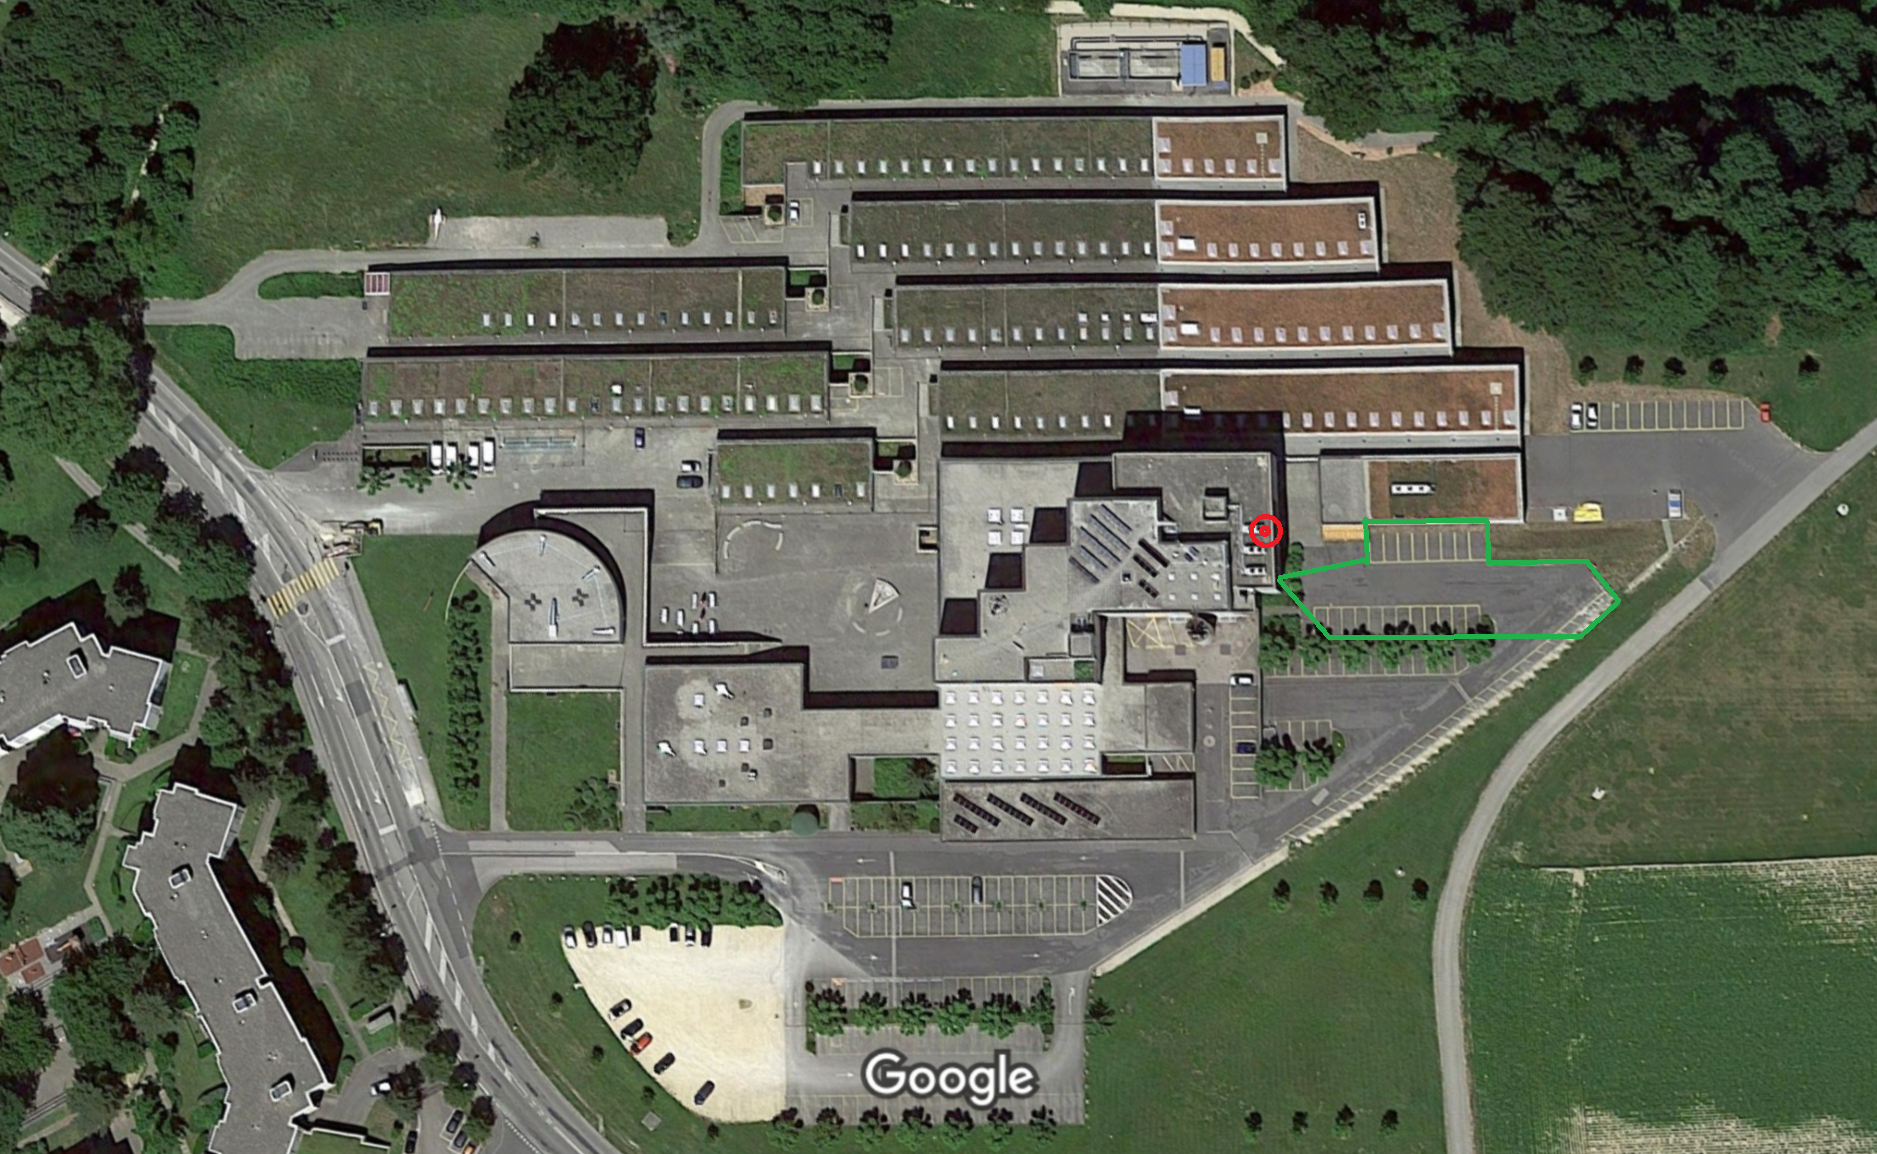
\includegraphics[width=14cm]{img/conception/cam_parking_location.png}
    \centering
    \captionsource{Emplacement de la caméra (en rouge) et du parking filmé (en vert)}{map:heig-vd}
    \label{fig:cam_parking_annotation}
\end{figure} 

Y est désigné par un cercle rouge l'emplacement de la caméra. Elle se situe sur la terrasse du bâtiment est, accessible au niveau K. Elle est orientée afin de pouvoir capturer des images du parking désigné en vert. 

Malheureusement, lors des tests effectués après réception de la caméra \textbf{Wanscam} \textit{HW0029-5}, il a été remarqué que le signal Wifi présent sur le toit n'était pas suffisamment fiable afin de connecter la caméra. Afin de palier à ce problème, un câble réseau Ethernet a tout de même pu être tiré de manière temporaire.

\subsection{Configuration des périphériques}
Dans cette sous-section, on trouvera des informations utiles concernant la caméra et la machine virtuelle. Ces informations seront utilisées dans la suite de ce rapport. 

Afin de pouvoir accéder à la caméra, un FQDN\footnote{\textit{FQDN}: \textit{Fully qualified domain name}, soit nom de domaine entièrement qualifié. \autocite{wiki:FQDN}} a été configuré. Celui-ci permet d'obtenir l'adresse IP de la caméra à l'aide du DNS local. Ainsi, plutôt que de s'adresser à elle par une adresse IP, il suffit d'utiliser en lieu et place l'adresse suivante:
\begin{center}
    \textit{ipcam.einet.ad.eivd.ch}
\end{center}

%\nomenclature{FQDN}{\textit{Fully qualified domain name}, soit nom de domaine entièrement qualifié}

Comme indiqué en section \ref{conception.architecture.capture.logique}, une VM est mise à disposition de ce projet afin de récupérer des images de la caméra. Son adresse IP, 10.192.75.100, est fixe.

\subsection{Requêtes et protocole}
La caméra \textbf{Wanscam} \textit{HW0029-5} expose un serveur web permettant sa configuration. Bien entendu, celui-ci permet des connexions authentifiées. Il utilise le protocole \textit{Basic Auth HTTP\footnote{Le protocole Basic Auth consiste à inclure dans les entêtes HTTP un champ \textit{Authorization}. Celui-ci contient le login et le mot de passe de l'utilisateur, sous forme encodée (\textit{Base64})}}\autocite{wiki:basic-auth}. Il est cependant important de remarquer que le serveur ne permet pas l'utilisation d'\textit{HTTPS}: ainsi, la connexion n'est pas chiffrée. Le mot de passe fournit à la caméra, bien qu'encodé, circule en clair sur le réseau. Il est  donc important de noter que dans le cadre d'une application professionnelle, ceci n'est pas envisageable.

Elle expose un \textit{endpoint} \textit{HTTP} permettant de récupérer l'image actuelle que filme la caméra. Ainsi, dans le cadre de ce projet, l'adresse \textit{http://ipcam.einet.ad.eivd.ch/web/tmpfs/snap.jpg} est utilisée. La figure \ref{fig:image_request} présente donc ce protocole de communication qui est utilisé afin de récupérer des images.

\begin{figure}[H]
    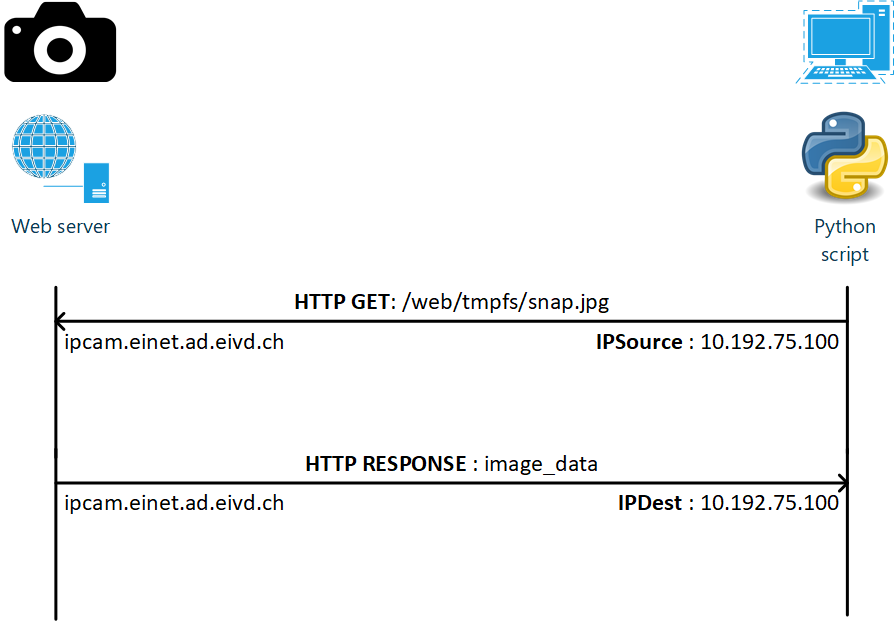
\includegraphics[width=130mm]{img/realisation/cam_request.png}
    \centering
    \caption{Requête d'une image à la caméra \textbf{Wanscam} \textit{HW0029-5}}
    \label{fig:image_request}
\end{figure} 

\subsection{Agent}\label{realisation.capture.agent}
Un agent a été développé, déployé sur la VM. Celui-ci permet de définir un intervalle auquel des images seront demandées à la caméra. Il permet donc de gérer la connexion à celle-ci, mais aussi les pertes de liaisons. A la réception d'une image, il permet de définir une méthode de traitement (décrite en section \ref{conception.traitement} et \ref{realisation.traitement}). 
Il permet aussi de définir, si tel est souhaité, une heure de début et une heure de fin durant lesquelles les requêtes seront effectuées. Lorsqu'on sort de cet intervalle, aucune photo ne sera capturée. Dans notre cas, celui-ci est utilisé afin d'éviter une multitude d'images prises du parking vide aux heures de nuit.

On trouvera au listing \ref{lst:agent} la création en python de celui-ci. Il faut remarquer qu'il n'a pas été souhaité de préciser les constantes \lstinline[columns=fixed]{USERNAME} et \lstinline[columns=fixed]{PASSWORD} pour des raisons de confidentialité. Il est aussi nécessaire de préciser que \lstinline[columns=fixed]{handle_image} est la fonction qui décrit le traitement effectué sur chaque image reçue. Celle-ci sera décrite en section \ref{realisation.traitement}

% spellcheck-language "en"
\begin{lstlisting}[caption={Création d'un agent récupérant les images}, label={lst:agent}] 
CAMERA_HOST = "ipcam.einet.ad.eivd.ch"
IMAGE_REQUEST_MIN_DELTA = 60
IMAGE_REQUEST_START_TIME = time(4, 30) # Start time at  4h30 AM
IMAGE_REQUEST_STOP_TIME = time(23) # Stop time at 11 PM
# [...]

# Creating a camera client
camera = CameraClient(CAMERA_HOST, USERNAME, PASSWORD)
# Creating a agent which requests the camera for an image once every hour
agent = CameraAgent(camera, handle_image, minutes = IMAGE_REQUEST_MIN_DELTA, running_time=(IMAGE_REQUEST_START_TIME, IMAGE_REQUEST_STOP_TIME))
\end{lstlisting}
% spellcheck-language

Ainsi, une image sera demandée toutes les heures, de 4h30 à 11h.

\subsection{Monitoring}
La caméra utilisée fonctionne sur batterie et panneaux solaires. Ainsi, il a semblé important de pouvoir surveiller le bon fonctionnement du système, et d'être averti en cas de malfonctionnement afin de pouvoir agir au plus vite. On pensera notamment à une perte de connexion due à des batteries faibles (par exemple, suite à un manque de soleil sur plusieurs jours consécutifs), ou encore à un câble déconnecté.

\textit{Python} offre un système complet natif de journalisation. Lorsque ce système est utilisé dans les modules créés, il est aisé de traiter des logs, et même d'avertir par mail des erreurs produites. Ce module peut être importé grâce à l'instruction \lstinline[columns=fixed]{import logging}.

Ce système offre plusieurs niveau de log. On les trouvera ci-dessous, du plus critique au moins important\autocite{doc:log}:
\begin{itemize}
    \item \lstinline[columns=fixed]{CRITICAL}
    \item \lstinline[columns=fixed]{ERROR}
    \item \lstinline[columns=fixed]{WARNING}
    \item \lstinline[columns=fixed]{INFO}
    \item \lstinline[columns=fixed]{DEBUG}
    \item \lstinline[columns=fixed]{NOTSET}
\end{itemize}

Ainsi, le niveau de chacun des logs effectués lors de la capture d'image a été défini. Une liste des logs importants concernant ce monitoring est proposée ci-dessous:
\begin{description}
    \item[INFO] Une image a été capturée et bien reçue
    \item[ERROR] La connexion à la caméra a été perdue
    \item[INFO] La caméra n'est toujours pas accessible
    \item[WARNING] La connexion à la caméra a été rétablie
\end{description}

\textit{Python} permet d'écouter les logs émis par un module. Il est aussi possible de définir le niveau d'écoute. Par exemple, il peut être souhaité de capturer tous les logs de niveau \textit{WARNING}. Dans ce cas, tous les logs de ce type seront capturés, ainsi que tous les logs dont le niveau est supérieur (soit plus important). 

Lors de l'arrivée d'un log, un système de \textit{handler} (proposé par \textit{Python}) a été mis en place. On en distinguera 3:
\begin{description}
    \item[Terminal handler] Ecoute les logs à partir du niveau \textit{INFO}. A l'arrivée d'un log, celui-ci est affiché dans la console. Les informations de debug ne sont pas affichées.
    \item[File handler] Ecoute tous les logs. Ainsi, une trace est gardée de tous les logs dans le système de fichier. Ce gestionnaire est de type \lstinline[columns=fixed]{TimedRotatingFileHandler}, qui permet de créer un nouveau fichier de logs par jour. 
    \item[SMTPHandler] Ecoute les logs à partir du niveau \textit{WARNING}. Lors d'une erreur ou d'un avertissement, un mail est envoyé automatiquement.
\end{description}

Ainsi, il est possible d'agir rapidement lors d'une perte de connexion à la caméra. Le log associé étant de type (\textit{ERROR}), un mail est envoyé à l'aide du \textit{SMTPHandler}. Si la caméra est reconnectée (\textit{WARNING}), un mail est aussi reçu.

\section{Traitement des images}\label{realisation.traitement}

La figure \ref{fig:image_process} présente la récupération et le traitement des images qui est effectué.

\begin{figure}[H]
    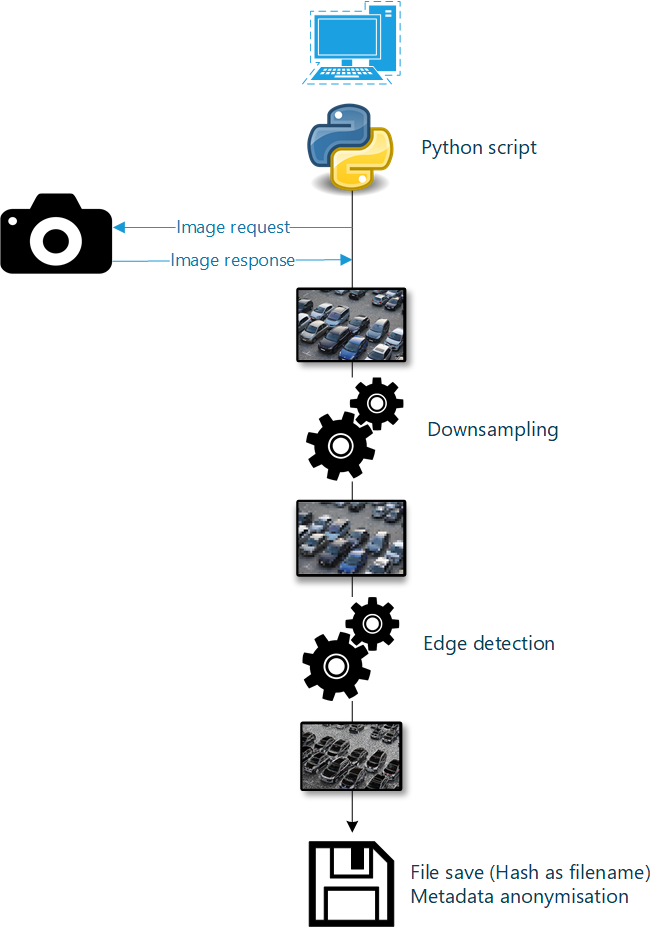
\includegraphics[width=110mm]{img/realisation/image_process.png}
    \centering
    \caption{Requêtes d'images et traitement}
    \label{fig:image_process}
\end{figure} 

Dans un premier temps, un script Python interroge la caméra et récupère une image tel qu'il a été décrit en section \ref{realisation.capture} précédente. Ensuite, l'image est sous-échantillonnée, et les bords détectés. Pour ce faire, \textit{Scikit-image} a été utilisé.

Le code \ref{lst:handling_image} présenté montre la méthode traitant les images entrantes. Celles-ci sont passées en argument de la méthode (\lstinline[columns=fixed]{image_stream}).


% spellcheck-language "en"
\begin{lstlisting}[caption={Traitement des images reçues}, label={lst:handling_image}] 
# Defining what to do when an image is received
def handle_image(image_stream):
    # Converting to a skimage/opencv image (simply a [x, y, 3] numpy array)
    image = io.imread(image_stream)

    # Firstly, downsampling the image
    image = transform.resize(image, IMAGE_OUTPUT_SIZE, mode='reflect', anti_aliasing=True)

    # Secondly, detecting the edges
    image = scharr_hsv(image)

    # Then, we output the image to the folder
    # We use a hash as an ID
    # We could have used a datetime format as a unique filename, but this could results to a lack of privacy
    # Saving it as a bitmap: no decompression to do when loading a lot of file
    # Note: hashing time is negligible
    h = hash(image.data.tobytes())
    filename = IMAGE_FOLDER + hex(h)[-15:] + ".bmp"

    with warnings.catch_warnings(): # used to ignore loss of precision warning
        warnings.simplefilter("ignore")
        io.imsave(filename, image)

    # We then have to reset metadata access and edit time because of privacy issues
    os.utime(filename, (946684800, 946684800))
\end{lstlisting}
% spellcheck-language

La méthode \lstinline[columns=fixed]{_scharr_hsv} utilisée est décrite au listing de code \ref{lst:scharr_filter}. 

Il est possible d'y distinguer la ligne \lstinline[columns=fixed]{@adapt_rgb(hsv_value)}, 

provenant de la librairie \textit{scikit-image}. Elle permet d'adapter le filtre \textit{scharr} présent dans la méthode sur chacun des canaux de l'image.

% spellcheck-language en
\begin{lstlisting}[caption={Détection de bord à l'aide de \textit{scikit-image}}, label={lst:scharr_filter}] 
@adapt_rgb(hsv_value)
def _scharr_hsv(image):
    return filters.scharr(image)
\end{lstlisting}
% spellcheck-language

Dans le cadre de l'anonymisation des données, il a semblé important qu'aucune information concernant les utilisateurs puisse apparaître. C'est pourquoi le nom de l'image est basé sur son hash (fonction de hash fournie par Python. Un hash complexe n'est pas nécessaire). 

L'image est ensuite sauvegardée à un format \textit{bitmap} (\textit{.bmp}), sans pertes de compression. La date et l'heure de création et de modification du fichier sont aussi modifiées pour que les données soient au plus anonymisées.

\section{Traitement du corpus \textit{PKLot}} \label{realisation.dataset}

Les images fournies par \textit{PKLot} sont annotées par place de parc marquée au sol. Cependant, il est possible que certaines voitures ne soient pas stationnées sur l'une de celle-ci. 

Si lors de l'entrainement, l'image segmentée par place de parc est utilisée, cela ne poserait aucun problème. Cependant, dans le cadre de ce projet, les modèles sont entrainés sur l'ensemble de l'image. Ainsi, certaines voitures présentes n'ont pas été annotées comme telles. Si ce \textit{dataset} n'était pas traité, certaines voitures seraient considérés comme étant de l'arrière-plan, et ne seraient pas détectée. 

\begin{figure}[ht]
    
    \begin{subfigure}{\textwidth}
        \centering
        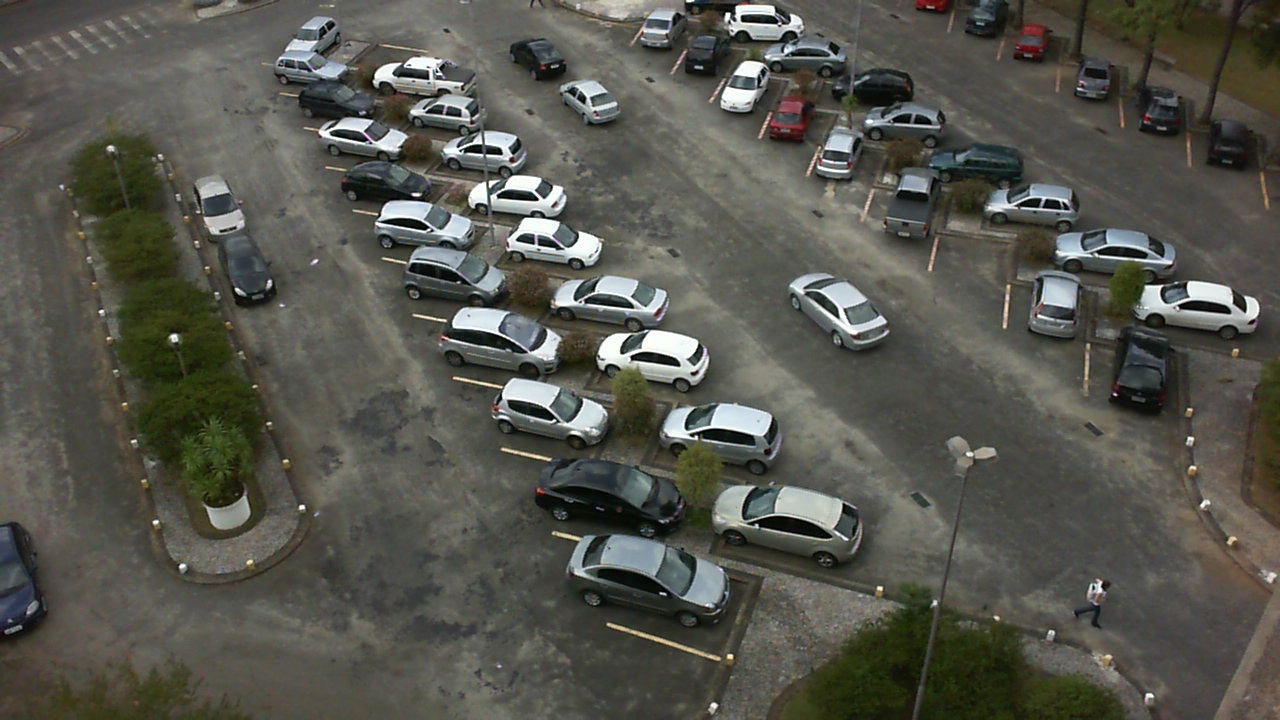
\includegraphics[width=.6\linewidth]{img/realisation/fill_before.jpg}
        \caption{Avant remplissage}
    \end{subfigure}%   

    \bigskip
    \begin{subfigure}{\textwidth}
        \centering
        
\includegraphics[width=.6\linewidth]{img/realisation/fill_mask.png}
        \caption{Masque utilisé}
    \end{subfigure}

    \bigskip
    \begin{subfigure}{\textwidth}
        \centering
        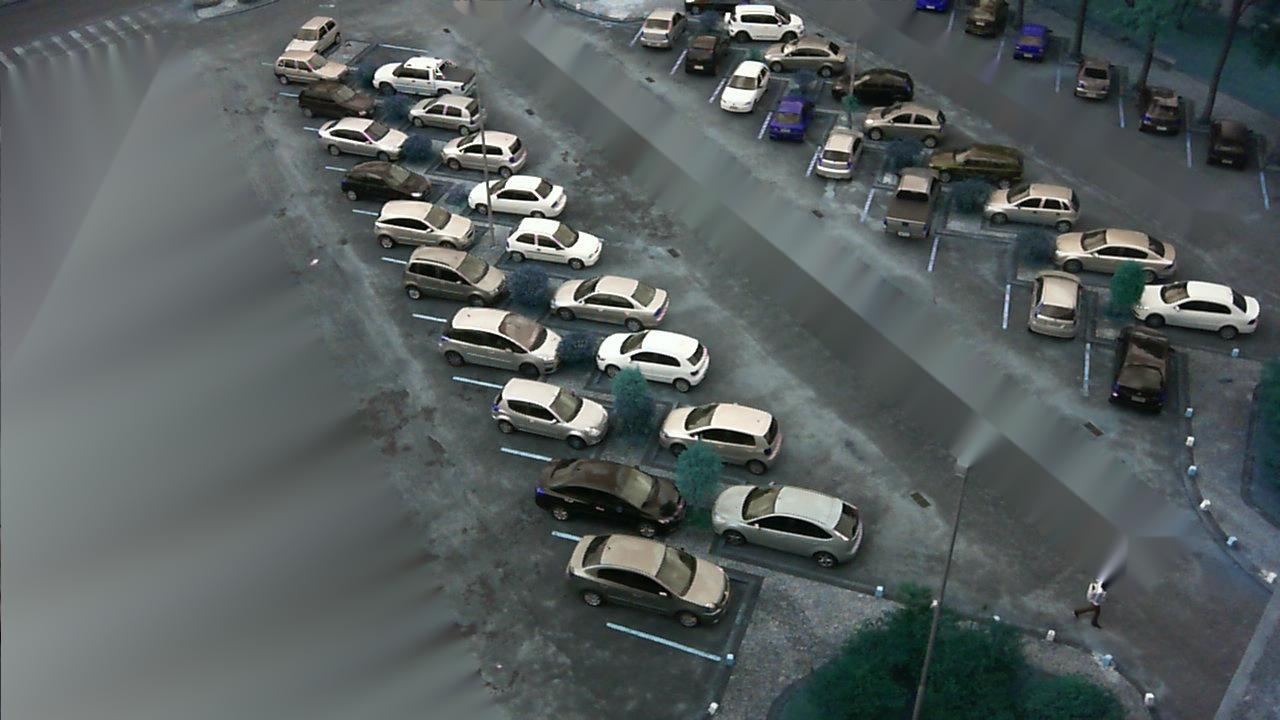
\includegraphics[width=.6\linewidth]{img/realisation/fill_after.jpg}
        \caption{Après remplissage}
    \end{subfigure}

    \caption{Avant-après traitements d'une image du corpus \textit{PKLot}}
    \centering
    \label{fig:image_fill_compare}
\end{figure}

Le corpus \textit{PKLot} est séparé en 3 dossiers différents pour chacune des caméras disponibles. Chaque image a été traitée à l'aide d'une méthode de remplissage, permettant d'effacer certaines régions d'une image\autocite{wiki:inpainting}. Pour ce faire, \textit{OpenCV} a été utilisé. La figure \ref{fig:image_fill_compare} en présente un résultat.

Il faut noter qu'un remplissage de qualité n'est pas nécessaire. En effet, il est avant tout nécessaire d'effacer les voitures présentes qui n'ont pas été annotée comme telles. 

Par la suite, les entrainements qui ont été effectués utilisent l'ensemble de ces images traitées, sans distinction entre les caméras. Cela permet d'augmenter la généralisation des modèles générés.

\section{Mise en place et entrainements des modèles}

\subsection{Machine virtuelle}
Afin d'obtenir de meilleures performances pour l'entrainement des modèles, une machine virtuelle a été créée sur \textit{AWS} \footnote{\textit{AWS}, pour \textit{Amazon Web Service}, fourni un système de IaaS (\textit{Infrastructure as a Service} où il est possible, entre autres, d'instancier des machines virtuelles puissantes). \url{https://aws.amazon.com/}}. Elle fournit aussi des images d'instances spécialisées dans le \textit{Machine learning}, où par exemple \textit{TensorFlow} et \textit{Keras} sont préinstallés\footnote{Les images sont disponibles à l'adresse \url{https://aws.amazon.com/fr/machine-learning/amis/}.}. C'est celle-ci qui a été utilisée. Les corpus d'images nécessaires à l'entrainement y ont été téléchargés et pré-traités à l'aide de scripts \textit{Python} qui ont été développé dans le cadre de ce projet.

\subsection{Format \textit{VOC} \textit{XML}}
Un format courant d'annotations d'images est le format \textit{VOC}, qui permet une certaine interopérabilité. Un exemple en est donnée au code \ref{lst:voc}. Le nom de l'image ainsi que sa taille y est indiqué, Aussi, chaque objet présent dans l'image y est indiqué, ainsi que sa classe et sa \textit{bounding box} associée. Il y a un fichier \textit{VOC} par images.

% spellcheck-language "en"
\begin{lstlisting}[caption={Exemple de fichier \textit{VOC}}, label={lst:voc}, language=XML] 
<annotation>
<filename>2012-11-10_07_12_40.jpg</filename>
<size>
    <width>1280</width>   
    <height>720</height>
    <depth>3</depth>
</size>
<segmented>0</segmented>
<object>
    <name>car</name>
    <bndbox>
        <xmin>669</xmin>
        <ymin>419</ymin>
        <xmax>717</xmax>
        <ymax>475</ymax>
    </bndbox>
</object>
</annotation>
\end{lstlisting}
% spellcheck-language

Les annotations fournies par \textit{PKLot} sont dans un format \textit{XML} qui leurs sont propres. Il a été nécessaire de transcrire ces \textit{XML} au format \textit{VOC}. Pour ce faire, un script \textit{Python} a été utilisé. Celui-ci utilise la librairie \textit{etree} pour \textit{parser} le fichier original, et en créer un nouveau correspondant au format \textit{VOC} voulu. 

\subsection{\textit{Tensorflow Object Detection API}}
Comme précédemment indiqué dans ce rapport, l'API de détection d'objets fournie par \textit{Tensorflow} a été utilisée. Celui-ci n'étant pas inclus dans \textit{TensorFlow}, le \textit{repo}\footnote{On trouvera le repo sur \url{https://github.com/tensorflow/models/tree/master/research/object_detection}} de l'API a été cloné et utilisé. Il a été nécessaire de l'ajouter aux variables d'environnements \textit{Python} afin qu'il soit possible d'importer directement les librairies nécessaires depuis un script \textit{Python}.

Afin d'utiliser un corpus d'entrainement à l'aide de \textit{Tensorflow}, des fichier \textit{.record} doivent être généré. Ceux-ci contiennent les images et leurs annotations. Ils peuvent être aisément créés à partir de fichiers \textit{VOC} à l'aide de la librairie \textit{TensorFlow} et d'un script \textit{Python}. 

Un fichier de configuration (\textit{.config}) est aussi nécessaire. Celui-ci indique où se situe les fichiers \textit{.record}, le modèle pré-entrainé, etc. Par la suite, l'entrainement est exécuté en ligne de commande.

% spellcheck-language "en"
\begin{lstlisting}[caption={Exécution d'un entrainement à l'aide de \textit{Tensorflow Object Detection API}}, label={lst:cmd_train}, numbers=none] 
python /home/ubuntu/tensorflow_models/research/object_detection/train.py \
--logtostderr \
--train_dir=/home/ubuntu/DS/PKLot/tensorflow_ds/training/ \
--pipeline_config_path=/home/ubuntu/TB/GIT/dev/park_python/drafts/object_detection/tensorflow_api_pklot/training.config
\end{lstlisting}
% spellcheck-language

\subsection{\textit{Yolo}}
Une implémentation de \textit{Yolo} a aussi été utilisée. Pour ce faire, il a été nécessaire de télécharger le code source du réseau de neurones open-source \textit{Darknet}\autocite{lib:yolo}, en clonant le \textit{repo} associé.

Une fois celui-ci téléchargé, l'attribut \textit{OPENMP} du fichier \textit{Makefile} a été défini à 1 afin que les entrainements puissent être effectués sur tous les cœurs de la machine disponible. Puis, le code a été compilé à l'aide de la commande \textit{make} linux. Il faut noter que cette commande n'est pas nativement disponible sous Windows.

Dans un second temps, il est nécessaire de préparer les labels pour l'entrainement. Puisque les formats \textit{VOC} ont été créés pour le corpus \textit{PKLot}, un script \textit{Python} fourni par \textit{Darknet} a été utilisé. Les fichiers de configurations nécessaires à l'entrainement sur le \textit{dataset} ont aussi été modifiés. 

\begin{lstlisting}[caption={Exécution d'un entrainement à l'aide de \textit{Yolo}}, label={lst:yolo_train}, numbers=none] 
./darknet detector train cfg/coco.data cfg/yolov3.cfg darknet53.conv.74
\end{lstlisting}
% spellcheck-language


\section{Utilisation du modèle final \textit{Tensorflow}} 
Comme l'indique les tests en section \ref{tests.final} \itnameref{tests.final}, un modèle utilisant l'API de \textit{Tensorflow} a été choisi. 

Une classe, \textit{TensorflowPredictor}, a été créée, basée sur des codes d'exemples disponibles (dont les sources sont précisées dans le code source). Lors de son instanciation, le chemin vers le modèle qu'on souhaite utiliser est passé en paramètre, ce qui a pour effet de le charger en mémoire. Ensuite, il est possible d'utiliser cet objet afin de prédire le nombre de voitures présentes sur une image. Le script permet aussi une exécution en ligne de commande afin de pouvoir générer les \textit{bounding box} d'une image.

\chapter{Tests et validation}\label{tests}
Ce chapitre permet d'évaluer et comparer les modèles de détections d'objets \textit{faster RCNN} et \textit{Yolo v3}, tels que décrits en section \ref{conception.model.object} \itnameref{conception.model.object}. Il est important de noter qu'il a été remarqué qu'en général, la détection d'objets repose sur un entrainement à l'aide des images où la détection de bord n'a pas été effectuée. Aussi, quelques entrainements ont été effectués sur les images traitées, qui n'ont apportés aucun résultat concluant. C'est pourquoi seul le corpus \textit{PKLot} (pré-traité à l'aide d'un remplissage de région tel qu'indiqué en section \ref{realisation.dataset}) est utilisé.

Ont été évalués:
\begin{itemize}
    \item Le modèle pré-entrainé.
    \item Le modèle ré-entrainé sur le corpus d'image \textit{PKLot} avec différents nombres d'itérations. Le nombre d'itérations nécessaires diffère en fonction des modèles utilisés.
\end{itemize}

Chacun des modèles pré-cités ont été évalués à l'aide de la méthode décrite en section \ref{conception.eval} \itnameref{conception.eval}. 

\section{TensorFlow Object Detection API}
Le modèle \textit{Faster RCNN} a été évalué à l'aide de l'API de détection d'objets de \textit{TensorFlow}. On trouvera en figure \ref{fig:tensorflow_train} l'entrainement qui a été effectué sur le corpus d'images \text{PKLot}.

\begin{figure}[H]
    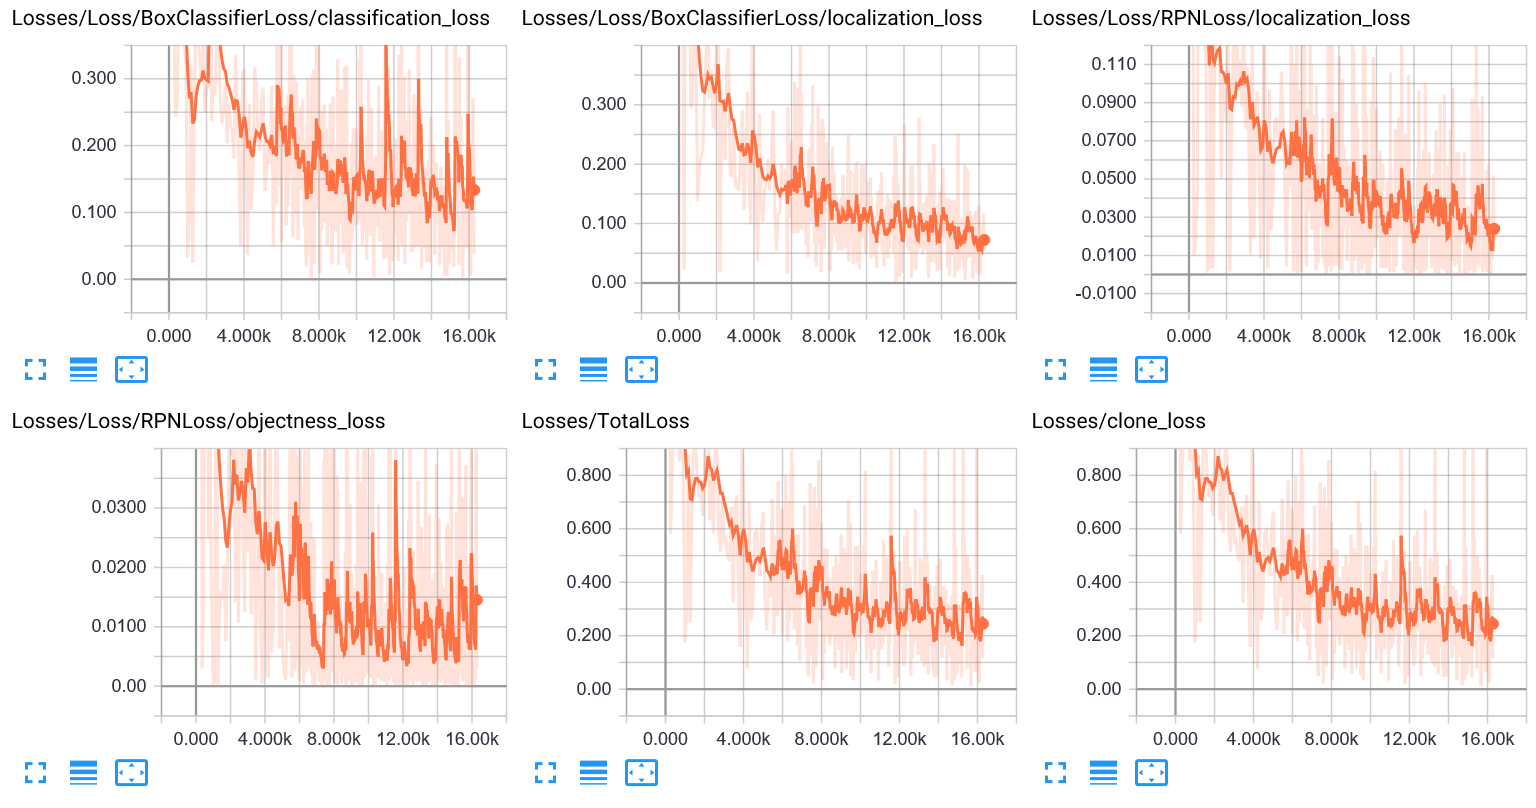
\includegraphics[width=15cm]{img/tests/tensorflow_pklot_full_train.png}
    \centering
    \caption{Entrainement sur le corpus \textit{PKLot} (graphes par \textit{Tensorboard})}
    \label{fig:tensorflow_train}
\end{figure} 

On distingue plusieurs fonctions objectifs:
\begin{description}
    \item[\textit{Classification loss}] La perte au fil des itérations lors de la classification. 
    \item[\textit{Localization loss}] Présente à quel point les \textit{bounding box} désignant les voitures sont bien localisées.
    \item[\textit{Objectness loss}] Pour chaque \textit{bounding box}, il s'agit de définir si c'est une voiture ou l'arrière-plan
    \item[\textit{Total loss}] Présente une combinaison des toutes les fonctions de pertes.
\end{description}

L'entrainement a été stoppé après 16000 itérations (plus de 2 jours de calculs). En effet, il semble qu'un certain palier ai été atteint. Aussi, plus d'itérations pourraient entrainer à un sur-apprentissage. Les nombres d'itérations 4000 et 16000 ont été évalués, ainsi que le modèle pré-entrainé.

Afin d'effectuer les tests, il est nécessaire de choisir un score minimum. Celui-ci indique, pour chaque objet détecté, à quel point l'algorithme est confiant sur sa prédiction. La figure \ref{fig:tensorflow_bb} présente une détection effectuée sur une image du \textit{dataset} \textit{PKLot}. 

\begin{figure}[ht]
    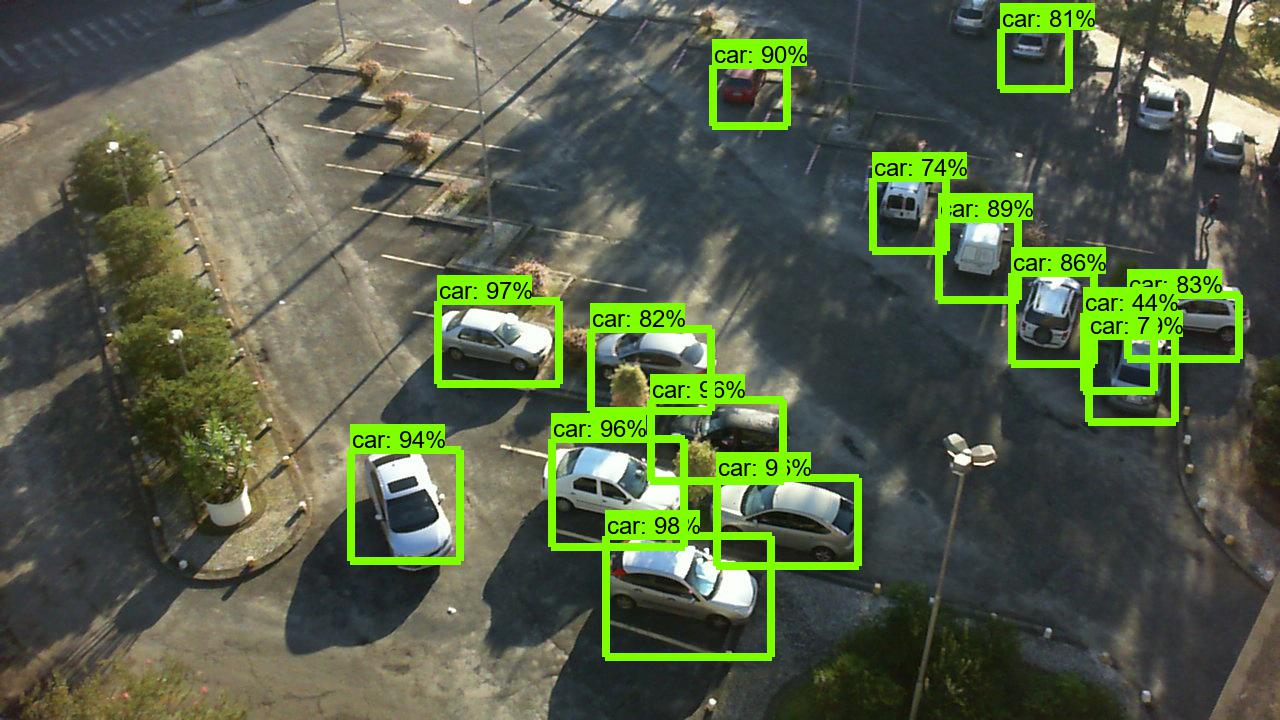
\includegraphics[width=10cm]{img/tests/tensorflow_bb.jpg}
    \centering
    \caption{Exemple de détection sur un entrainement de 4000 itérations}
    \label{fig:tensorflow_bb}
\end{figure} 

Les scores sont généralement supérieurs à 75\%. Il est possible de remarquer un faux positif d'un score de 44\%. Un seuil de 70\% a été défini, afin d'obtenir une certaine marge, et réduire le nombre de faux positif. Cependant, il faut remarquer que si le modèle \textit{Faster RCNN} est utilisé, ce seuil à du être abaissé à 20\% pour obtenir des résultats raisonnables. Ceci permet aussi d'indiquer que l'utilisation d'un modèle non ré-entrainé ne permet pas une grande confiance en l'algorithme.

\paragraph{Résultats}

Le tableau \ref{tab:rcnn_results} présente les résultats du modèles \textit{Faster RCNN} pré-entrainé (0 itérations), ainsi qu'entrainé avec 4000 et 1600 itérations supplémentaires sur le corpus d'images \textit{PKLot}. Les calculs qui ont été effectués ont été décrit en section \ref{conception.eval} \itnameref{conception.eval}.

\paragraph{\textit{Cars dataset}}

Un entrainement sur le \textit{dataset} \textit{Cars}, vu en section \ref{conception.dataset} \itnameref{conception.dataset}, a aussi été testé. Cependant, les résultats obtenus n'étaient pas bons, où un entrainement entrainait des résultats moins bon que le modèle pré-entrainé. Il est possible que ce corpus ne soit pas adapté pour des images de parkings, car les angles de vues prise des voitures et leurs tailles n'est pas similaire. Il n'a donc pas été souhaité de préciser les détails des résultats ici.

\begin{table}[ht]
\centering
\begin{tabular}{@{}ll@{}}
\toprule
N° itération & RMSE \\ \midrule
$0$            & $32.06564071$ \\
$4000$         & $10.4427355$ \\
$16000$        & $22.88589282$ \\ \bottomrule
\end{tabular}
\caption{\textit{Faster RCNN} - Résultats}
\label{tab:rcnn_results}
\end{table}

Le modèle entrainé 4000 fois semble le meilleur lors de l'évaluation. La cause est sans doute un sur-entrainement du modèle à 16000 itérations, ce qui ne permet pas de le généraliser suffisamment.

\section{Yolo v3}

Le modèle \textit{Yolo} a aussi été évalué. Un modèle pré-entrainé sur le corpus d'images \textit{Coco}\autocite{data:coco} à été utilisé.

\begin{figure}[ht]
    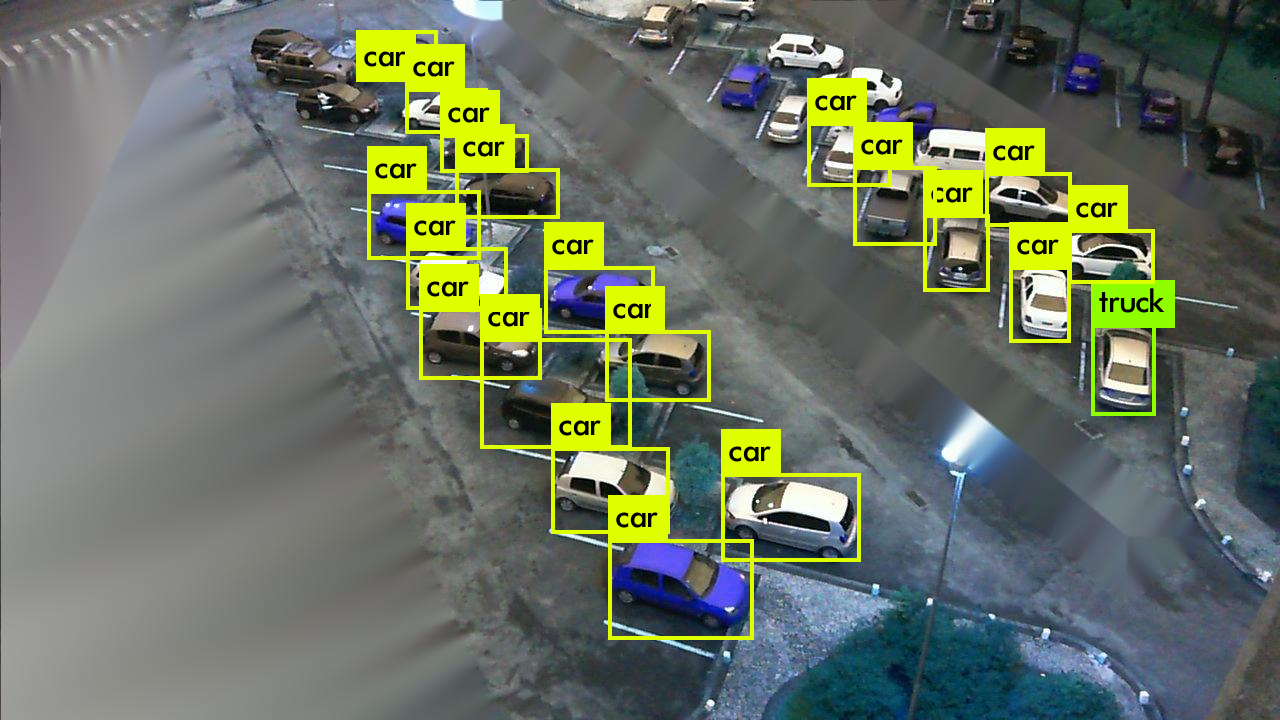
\includegraphics[width=10cm]{img/tests/yolo_bb.png}
    \centering
    \caption{Exemple de détection avec un modèle \textit{Yolo v3} pré-entrainé sur \textit{Coco}}
    \label{fig:yolo_bb}
\end{figure} 

Le réseau de neurones a aussi été entrainé sur le \textit{dataset} \textit{PKLot}, jusqu'à un nombre de 200 itérations. Cependant, les résultats n'ont pas été concluants, où que peu de voitures ont pu être détectées. 200 itérations semble un nombre très faible. Cependant, le temps d'entrainement nécessaires était trop grand, où moins de 100 itérations par jours étaient effectuées. Ainsi ici, aux vues des résultats médiocres, il n'a pas été souhaités de les intégrer à cette évaluations. Ainsi, seul le modèle pré-entrainé sur le corpus d'images \textit{Coco} a été effectué. 

De la même manière qu'auparavant, l'erreur au carré moyenne a été calculée sur le nombre de voiture détectées. On en trouvera le résultat en figure \ref{tab:yolo_results}.

\begin{table}[ht]
\centering
\begin{tabular}{@{}ll@{}}
\toprule
Modèle & RMSE \\ \midrule
Yolo v3 entrainé sur \textit{Coco}  & $34.75053725$ \\ \bottomrule
\end{tabular}
\caption{\textit{Yolo} - Résultats}
\label{tab:yolo_results}
\end{table}

\section{Choix final} \label{tests.final}

A la vues des résultats précédent, il semble que le meilleur algorithme soit le modèle \textit{Faster RCNN} ré-entrainé sur \textit{PKLot} avec 4000 itérations supplémentaires. Il faut noter que ces résultats ont été obtenus à l'aide du corpus d'images \textit{PKLot}: ainsi, certains paramètres, comme le seuil de détection, doit peut-être être modifié. 


\section{Tests en conditions réels}
Une fois le système mis en place (caméra, prédiction du taux d'utilisation, \textit{REST} API), il aurait été souhaité d'effectuer une évaluation approfondie de la détection des voitures. Cependant, pour cause de protection des données des utilisateurs du parking, seul quelques observations ont pu être effectuées. 

En général, il a pu être observé que le système semble viable, où seules 1 ou 2 voitures ne sont pas détectées. Il a pu être remarqué que le modèle ne détecte que très mal les voitures présentes sur le bord de l'image, où seul une partie de celle-ci est visible. 

Aussi, comme on pouvait si attendre, les voitures présentes derrière les arbres ne sont que très rarement jamais détectées, ceci dû à la verdure qui les cachent.  Ce n'est pas un problème en sois: il suffit de considérer le parking derrière les arbres comme ne faisant pas parti du parking dont on souhaite connaître l'état. Si il est tout de même souhaité que ces voitures doivent être détectées, il serait possible d'ajouter une seconde caméra.


\chapter{Conclusions}

\todo{Choix de la caméra pénible}



\begin{appendix}
\chapter{Résultats des traitements d'images}
\section{Sous-échantillonnages} \label{annexe.traitement.downsampling}

\begin{figure}[H]
    \centering
    \begin{subfigure}{.4\textwidth}
        \centering
        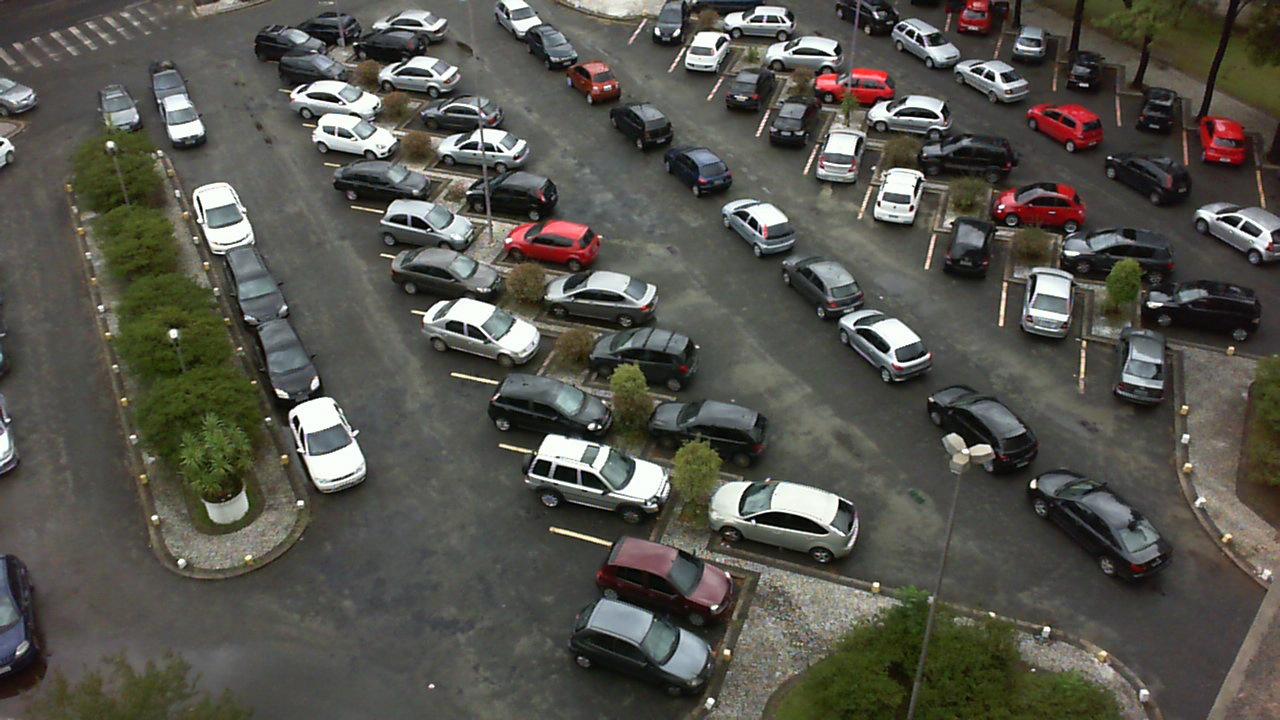
\includegraphics[width=.85\linewidth]{img/conception/image_process/downsample_only/7.png}
        \caption{1280 x 720}
    \end{subfigure}%
    \begin{subfigure}{.4\textwidth}
        \centering
        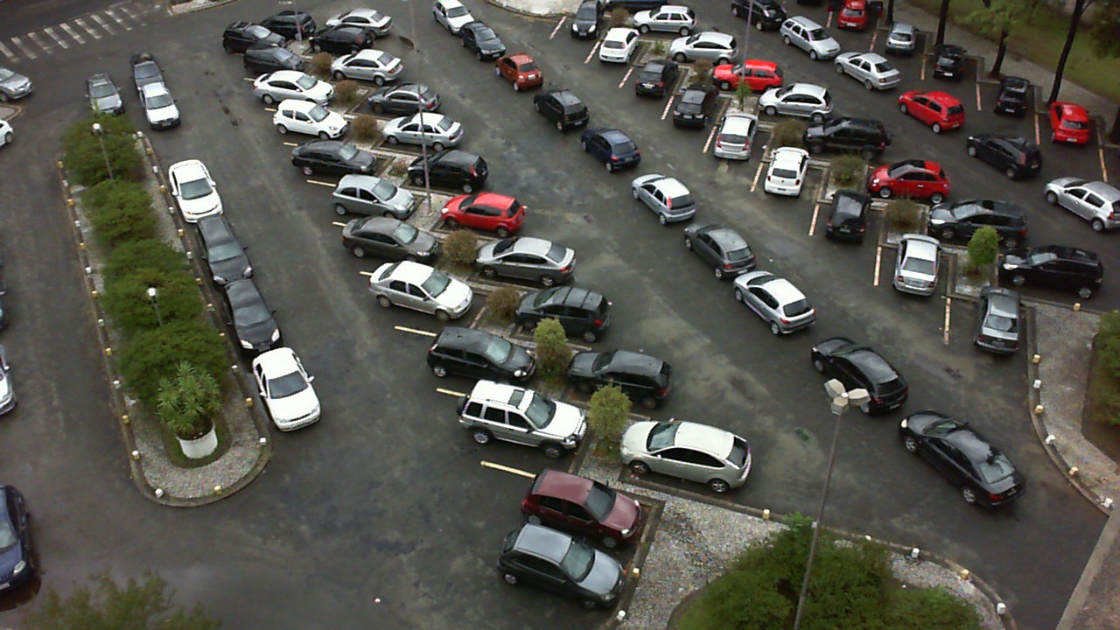
\includegraphics[width=.85\linewidth]{img/conception/image_process/downsample_only/6.png}
        \caption{1120 x 630}
    \end{subfigure}%   

    \bigskip
    \begin{subfigure}{.4\textwidth}
        \centering
        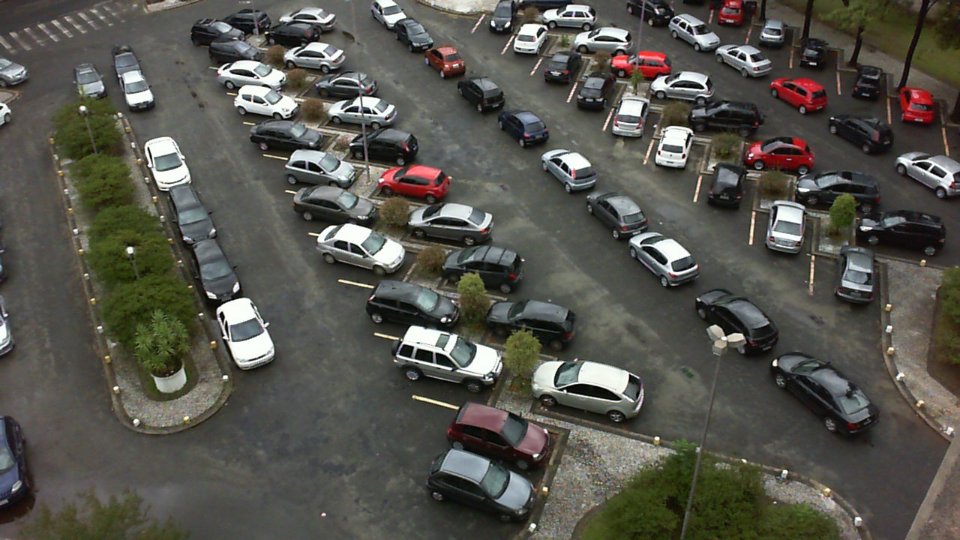
\includegraphics[width=.85\linewidth]{img/conception/image_process/downsample_only/5.png}
        \caption{960 x 540}   
    \end{subfigure}%   
    \begin{subfigure}{.4\textwidth}
        \centering
        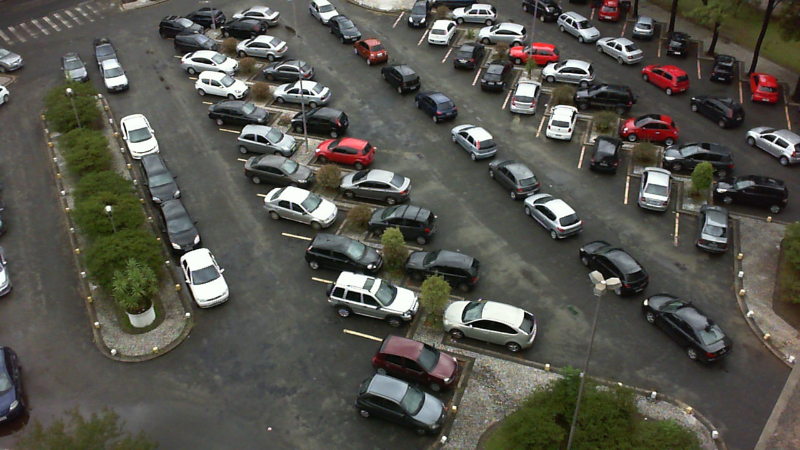
\includegraphics[width=.85\linewidth]{img/conception/image_process/downsample_only/4.png}
        \caption{800 x 450}
    \end{subfigure}% 

    \bigskip
    \begin{subfigure}{.4\textwidth}
        \centering
        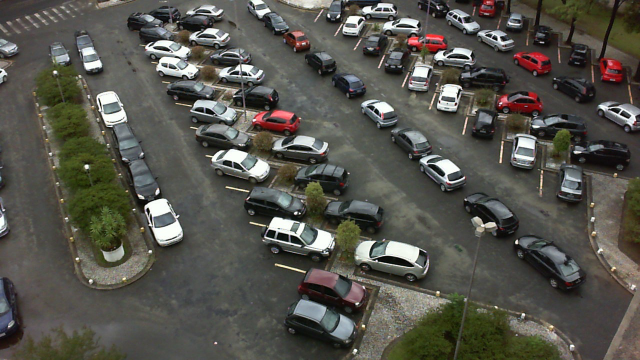
\includegraphics[width=.85\linewidth]{img/conception/image_process/downsample_only/3.png}
        \caption{640 x 360}
    \end{subfigure}%   
    \begin{subfigure}{.4\textwidth}
        \centering
        
\includegraphics[width=.85\linewidth]{img/conception/image_process/downsample_only/2.png}
        \caption{480 x 270}
    \end{subfigure}%  

    \bigskip
    \begin{subfigure}{.4\textwidth}
        \centering
        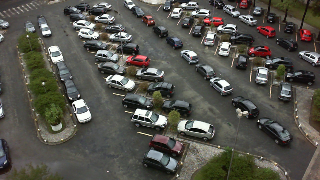
\includegraphics[width=.85\linewidth]{img/conception/image_process/downsample_only/1.png}
        \caption{320 x 180}
    \end{subfigure}%   
    \begin{subfigure}{.4\textwidth}
        \centering
        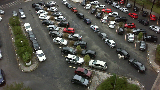
\includegraphics[width=.85\linewidth]{img/conception/image_process/downsample_only/0.png}
        \caption{160 x 90}
    \end{subfigure}%   
    \caption{L'image originale redimensionnée à différentes résolutions}
\end{figure}

\section{Détection de bords, sous-échantillonnage} \label{annexe.traitement.edge_down}
Ici, il est considéré que la détection de bord a été effectuée en premier, à l'aide d'un filtre \textit{Scharr} est appliqué sur l'espace HSV de l'image.

\begin{figure}[H]
    
\includegraphics[width=80mm]{img/conception/image_process/edges_only/5.png}
    \centering
    \caption{\textit{Scharr} HSV: image utilisée afin d'explorer les différents sous-échantillonnages}
    \label{fig:image_process_edge_down_orig}
\end{figure}

\begin{figure}[H]
    \begin{subfigure}{.5\textwidth}
        \centering
        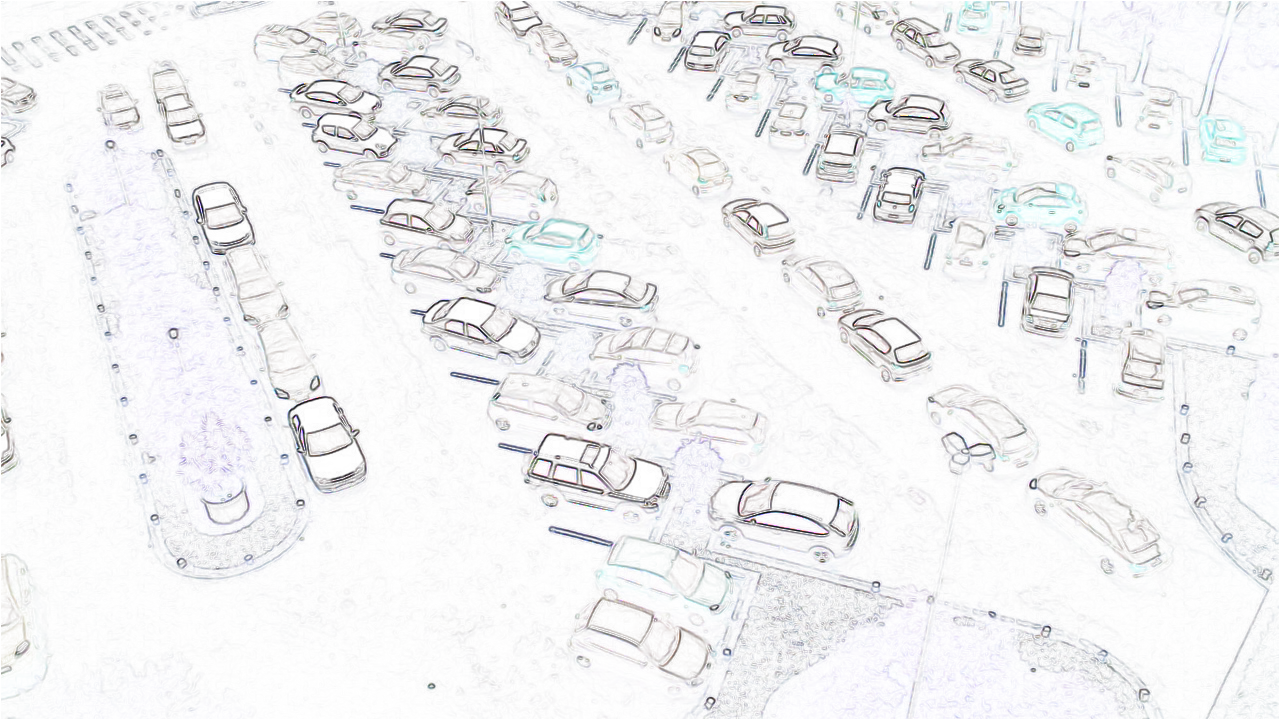
\includegraphics[width=.85\linewidth]{img/conception/image_process/edge-downsample/7.png}
        \caption{1280 x 720}
    \end{subfigure}%
    \begin{subfigure}{.5\textwidth}
        \centering
        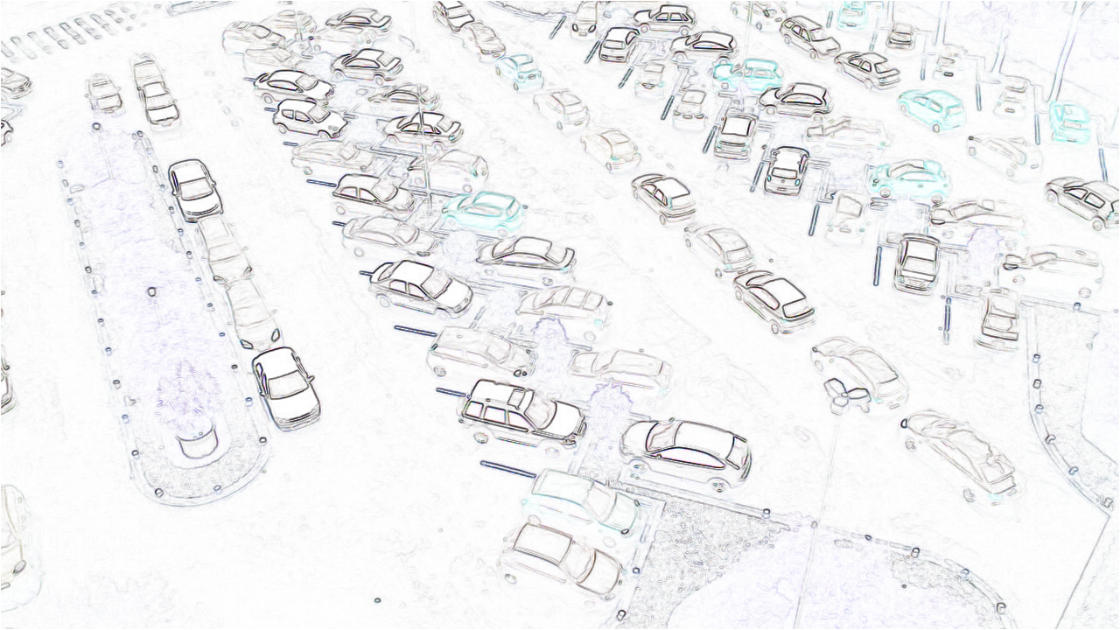
\includegraphics[width=.85\linewidth]{img/conception/image_process/edge-downsample/6.png}
        \caption{1120 x 630}
    \end{subfigure}%   

    \bigskip
    \begin{subfigure}{.5\textwidth}
        \centering
        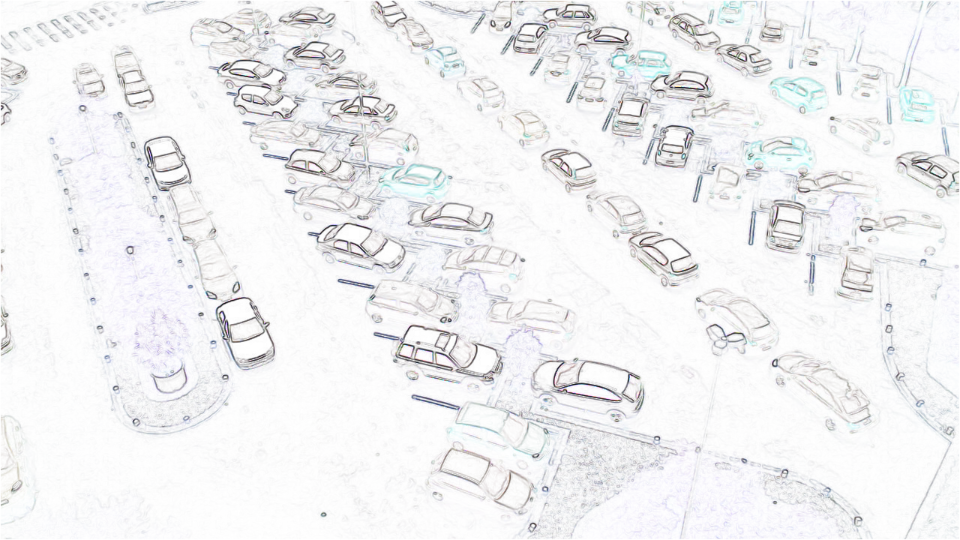
\includegraphics[width=.85\linewidth]{img/conception/image_process/edge-downsample/5.png}
        \caption{960 x 540}   
    \end{subfigure}%   
    \begin{subfigure}{.5\textwidth}
        \centering
        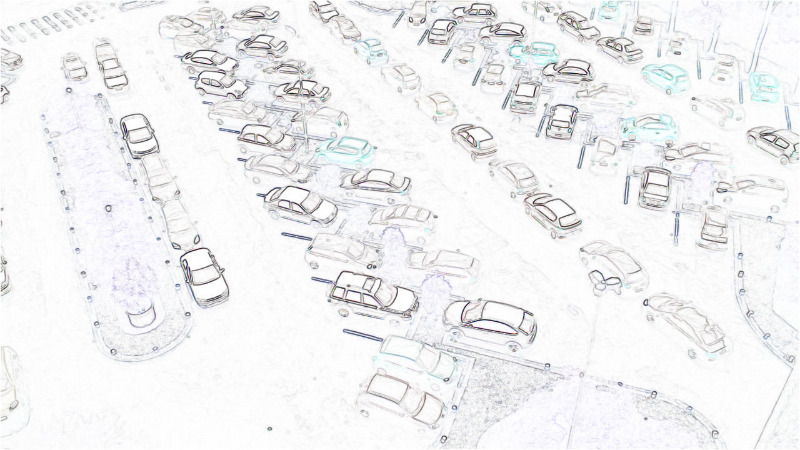
\includegraphics[width=.85\linewidth]{img/conception/image_process/edge-downsample/4.png}
        \caption{800 x 450}
    \end{subfigure}% 

    \bigskip
    \begin{subfigure}{.5\textwidth}
        \centering
        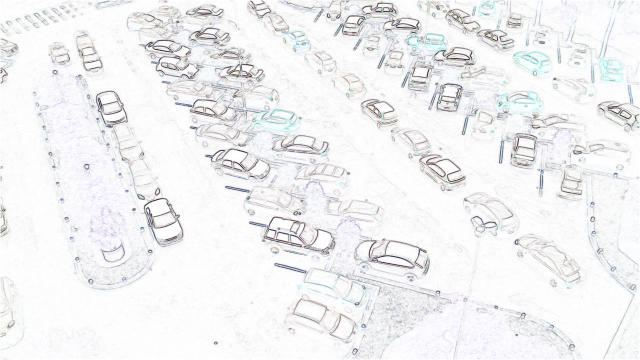
\includegraphics[width=.85\linewidth]{img/conception/image_process/edge-downsample/3.png}
        \caption{640 x 360}
    \end{subfigure}%   
    \begin{subfigure}{.5\textwidth}
        \centering
        
\includegraphics[width=.85\linewidth]{img/conception/image_process/edge-downsample/2.png}
        \caption{480 x 270}
    \end{subfigure}%  
    
    \bigskip
    \begin{subfigure}{.5\textwidth}
        \centering
        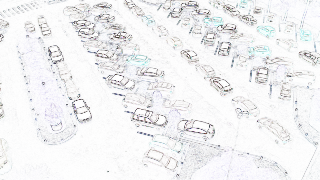
\includegraphics[width=.85\linewidth]{img/conception/image_process/edge-downsample/1.png}
        \caption{320 x 180}
    \end{subfigure}%   
    \begin{subfigure}{.5\textwidth}
        \centering
        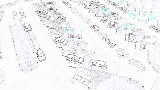
\includegraphics[width=.85\linewidth]{img/conception/image_process/edge-downsample/0.png}
        \caption{160 x 90}
    \end{subfigure}%   
    \centering
    \caption{L'image dont les bords ont été détectés, redimensionnée à différentes résolutions}
    \label{fig:image_process_edge_down}
\end{figure}

La figure \ref{fig:image_process_edge_down} applique plusieurs sous-échantillonnages de l'image \ref{fig:image_process_edge_down_orig}.

Il semble que l'image la plus légère et suffisamment précise afin de pouvoir détecter sans encombre des voitures est celle dont la résolution est de 480 x 270 pixels. Les images dont la taille est inférieure sont trop floues, où certaines voitures semblent parfois même disparaitre.


\section{Détection de bords, sous-échantillonnage} \label{annexe.traitement.down_edge}

Ce paragraphe présente les résultats d'un traitement qui consiste en sous-échantillonner l'image dans un premier temps, puis d'en détecter les bords. Lors des différents tests effectués, il a été remarqué qu'une résolution de 320x180 pixels, tel qu'indiqué dans le paragraphe \itnameref{conception.traitement.eval.downsample}, ne produisait pas des résultats concluants. C'est pourquoi la résolution de 480 x 270 pixels a été préférée. L'image utilisée est présentée en figure \ref{fig:image_process_down_edge_orig}.

\begin{figure}[H]
    
\includegraphics[width=110mm]{img/conception/image_process/downsample_only/2.png}
    \centering
    \caption{480 x 270: image utilisée afin d'explorer les différentes méthodes de détection de bords}
    \label{fig:image_process_down_edge_orig}
\end{figure}

\begin{figure}[H]
    \begin{subfigure}{.5\textwidth}
        \centering
        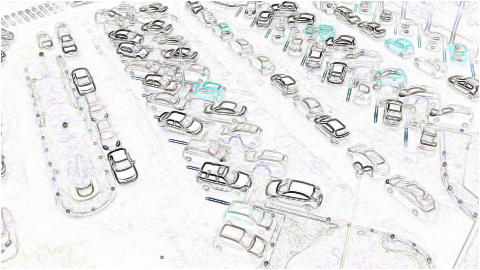
\includegraphics[width=.85\linewidth]{img/conception/image_process/downsample-edge/0.png}
        \caption{Filtre \textit{Sobel} - RGB}
    \end{subfigure}%   
    \begin{subfigure}{.5\textwidth}
        \centering
        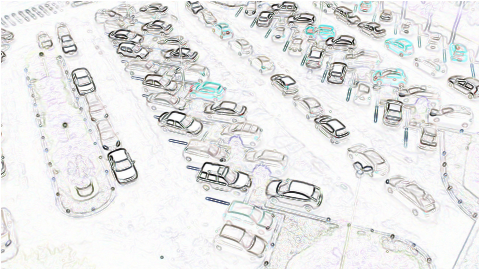
\includegraphics[width=.85\linewidth]{img/conception/image_process/downsample-edge/3.png}
        \caption{Filtre \textit{Scharr} - RGB}
    \end{subfigure}%  

    \bigskip
    \begin{subfigure}{.5\textwidth}
        \centering
        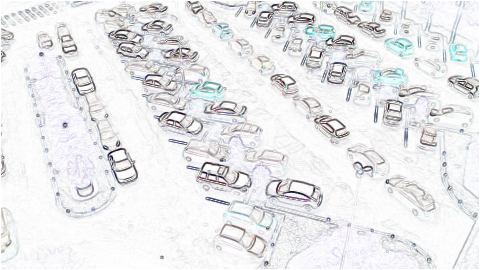
\includegraphics[width=.85\linewidth]{img/conception/image_process/downsample-edge/1.png}
        \caption{Filtre \textit{Sobel} - HSV}   
    \end{subfigure}%   
    \begin{subfigure}{.5\textwidth}
        \centering
        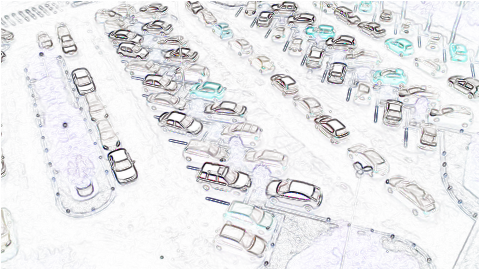
\includegraphics[width=.85\linewidth]{img/conception/image_process/downsample-edge/4.png}
        \caption{Filtre \textit{Scharr} - HSV}
    \end{subfigure}% 
    
    \bigskip
    \begin{subfigure}{.5\textwidth}
        \centering
        
\includegraphics[width=.85\linewidth]{img/conception/image_process/downsample-edge/2.png}
        \caption{Filtre \textit{Sobel} - Valeurs de gris}
    \end{subfigure}%   
    \begin{subfigure}{.5\textwidth}
        \centering
        
\includegraphics[width=.85\linewidth]{img/conception/image_process/downsample-edge/5.png}
        \caption{Filtre \textit{Scharr} - Valeurs de gris}
    \end{subfigure}%   
    \centering
    \caption{L'image sous-échantillonnée avec différentes détections de bords}
    \label{fig:image_process_down_edge}
\end{figure}

La figure \ref{fig:image_process_down_edge} présente l'application des différents filtres sur l'image sous-échantillonnées

Ici, de la même manière que décrit en annexe précédente \itnameref{annexe.traitement.down_edge}, le filtre semblant le mieux convenir est la matrice de convolution définie par \textit{Scharr} sur l'espace HSV. Les voitures y sont mieux distinguables, notamment grâce à leurs couleurs.

\chapter{Planification}
\begin{figure}[H]
    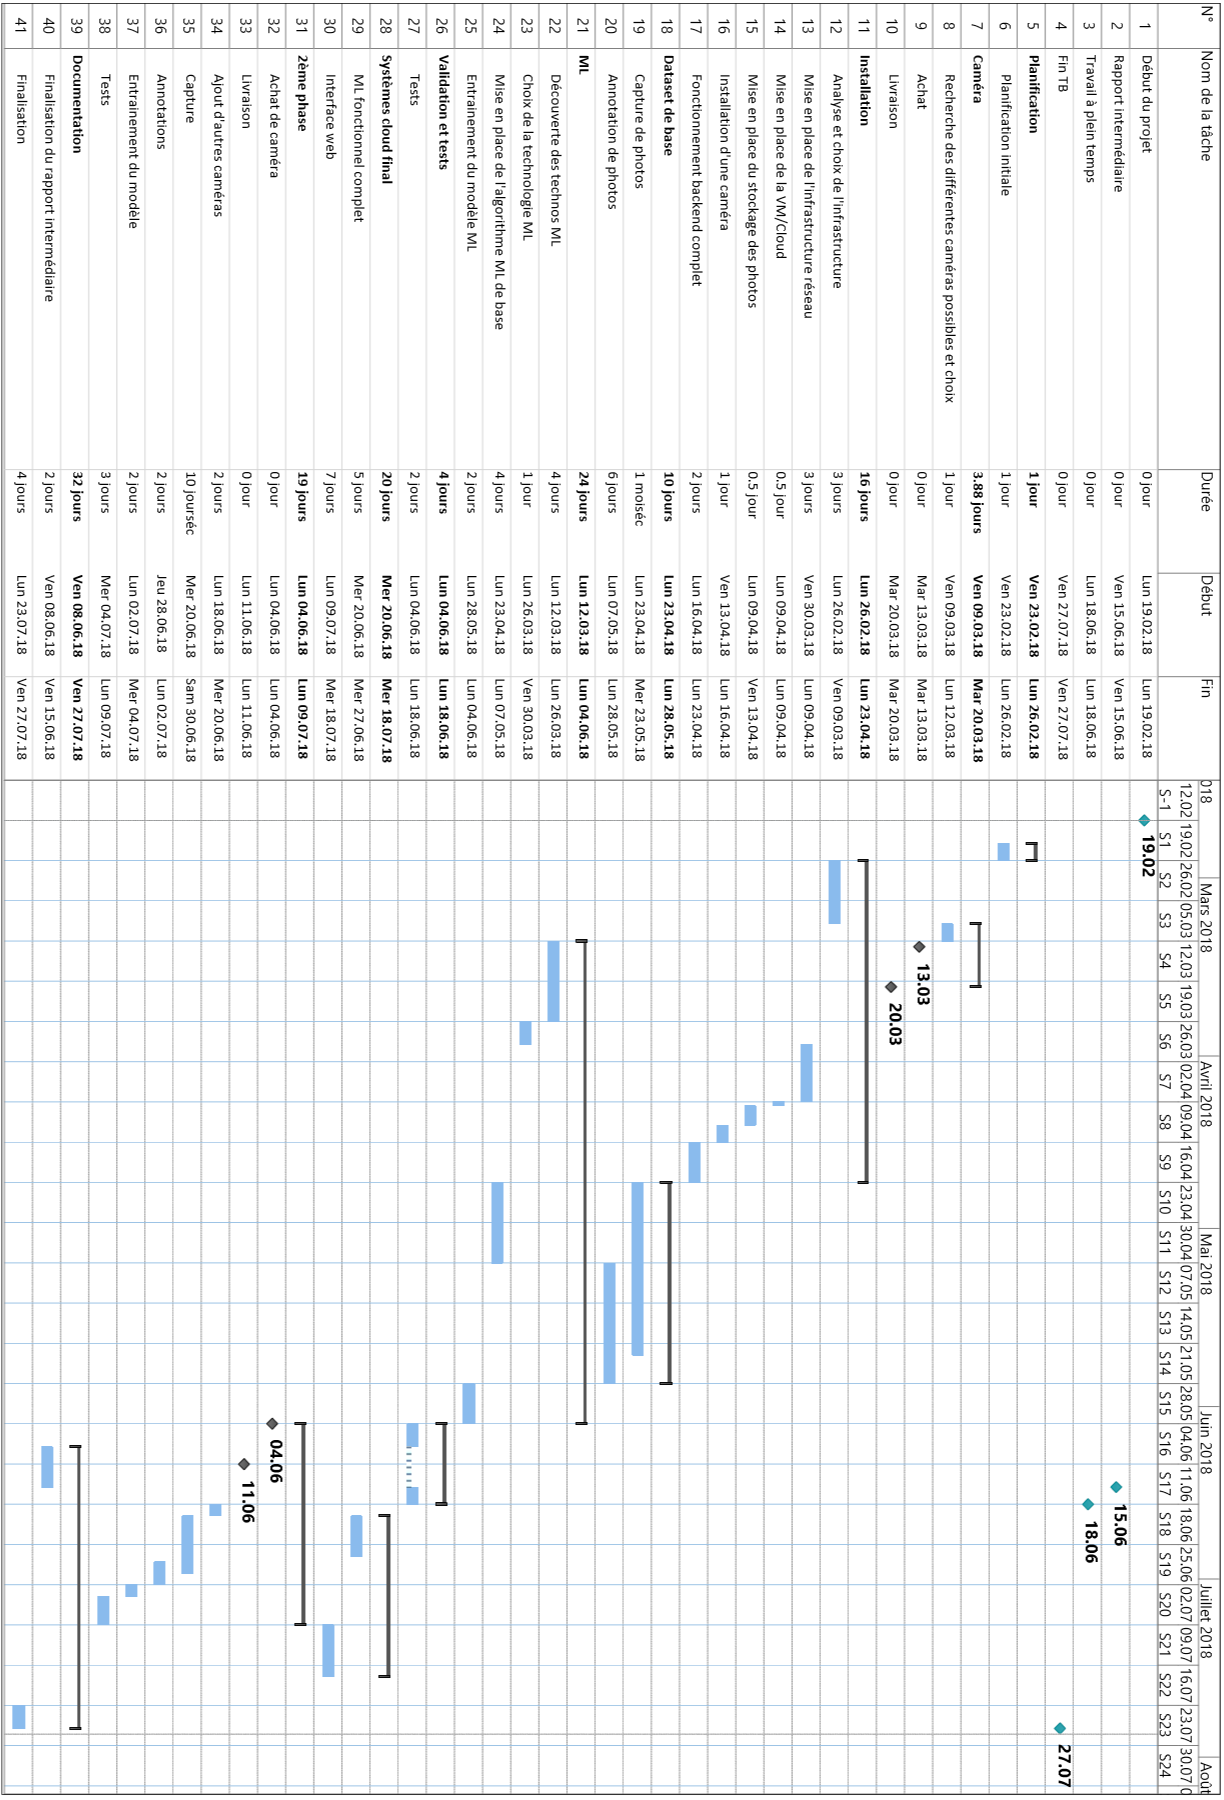
\includegraphics[width=14cm]{img/planif.png}
    \centering
\end{figure} 

\chapter{Réalisation}
\begin{figure}[H]
    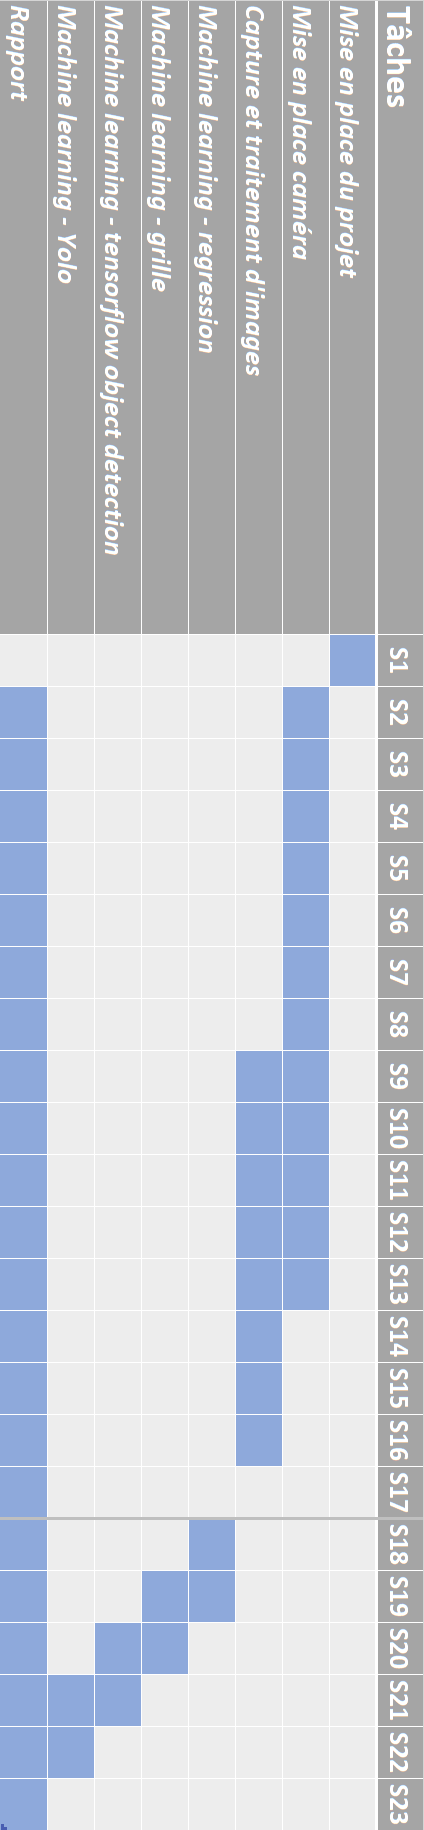
\includegraphics[width=4cm]{img/real.png}
    \centering
\end{figure} 

\end{appendix}

\chapter*{Outils utilisés}
\addcontentsline{toc}{chapter}{Outils utilisés}  

Dans le cadre de ce travail de Bachelor, plusieurs outils ont été utilisés à l'aide au développement et à la rédaction. On les trouveras dans ce chapitre.

\paragraph{Visual Studio Code}
\textit{Visual Studio Code}\footnote{\textit{Visual Studio Code}: https://code.visualstudio.com/} est un éditeur Open Source comparable à \textit{Sublime Text} ou \textit{Atom}. 

Il est possible d'y ajouter des extensions afin de convenir à l'usage souhaité. Dans ce projet, cet éditeur a été utilisé avant tout afin de coder en \textit{Python} et rédiger en \textit{LaTex}. Les extensions suivantes ont donc été installées:
\begin{description}
    \item[Python] Permet d'intégrer à VSCode le développement en Python. Propose un système de \textit{Linting}, \textit{debugging}, ou encore d'auto-complétion.
    \item[autoDocstring] Permet de générer automatiquement de la documentation python (\textit{Python Docstrings})
    \item[LaTex Workshop] Permet de compiler un projet \textit{LaTex}, proposant de la coloration de code, ou encore un système de \textit{preview} automatique.
    \item[BibTexLanguage] Permet d'ajouter au fichier de bibliographie \textit{.bib} une coloration syntaxique.
    \item[Spell Right] Permet la correction orthographique multi-langues de fichiers, dont les documents \textit{LaTex}.
\end{description}

\paragraph{VIM}
\textit{VIM} est un éditeur de texte en ligne de commande. Il a avant tout été utilisé afin d'effectuer des modifications mineurs de code sur la VM.

\paragraph{Conda}
Ce gestionnaire d'environnement a été choisi afin de pouvoir interpréter du \textit{Python} facilement. La commande \textit{pip install} a pu être utilisée afin d'installer aisément des librairies supplémentaires. Il faut noter que cette commande est plus du ressort de \textit{Python} que de \textit{Conda}

\paragraph{Git}
\textit{Git} est un gestionnaire de version distribué Open Source. Grâce à celui-ci, il a été possible de suivre l'évolution de la réalisation de ce TB. Un \textit{repository} associé à ce travail à été déployé sur \textit{Github}.

\paragraph{LaTex}
Le site \url{http://www.tablesgenerator.com/latex_tables} a été utilisé afin de pouvoir générer facilement des tables \textit{LaTex}.




\nocite{*}
\printbibliography
%\printnomenclature
%\printglossaries
 

\listoffigures
%\listoftables   

%\chapter*{Journal de travail}
\addcontentsline{toc}{chapter}{Journal de travail}  


\end{document}
